\documentclass{article}


\PassOptionsToPackage{numbers, compress}{natbib}


\usepackage[preprint]{neurips_2022}

% --- Korean translation support (xelatex + kotex) ---
\usepackage{kotex}
\usepackage{fontspec}
\setmainfont{NanumMyeongjo}[AutoFakeSlant=0.167]
\setsansfont{NanumGothic}[AutoFakeSlant=0.167]
\setmainhangulfont{NanumMyeongjo}[AutoFakeSlant=0.167]
\setsanshangulfont{NanumGothic}[AutoFakeSlant=0.167]
\setmonohangulfont{NanumGothicCoding}[AutoFakeSlant=0.167]
\setmonofont{NanumGothicCoding}[AutoFakeSlant=0.167]
\linespread{1.4}\selectfont
\renewcommand{\figurename}{그림}
\renewcommand{\tablename}{표}
\setlength{\parindent}{1.2em}
% --- end Korean support ---








% \usepackage[utf8]{inputenc} % (xelatex 사용으로 비활성화)
% \usepackage[T1]{fontenc}   % (xelatex 사용으로 비활성화)
\usepackage{hyperref}       %
\usepackage{url}            %
\usepackage{booktabs}       %
\usepackage{amsfonts}       %
\usepackage{nicefrac}       %
\usepackage{microtype}      %
\usepackage{xcolor}         %

\bibliographystyle{plainnat}

% \usepackage{times} % (xelatex+fontspec 사용으로 비활성화)
\usepackage{qtree}
\usepackage{latexsym}
\usepackage{microtype}
\usepackage{natbib}
\usepackage{booktabs}
\usepackage{appendix}
\usepackage{tikz}
\usepackage{tikz-dependency}
\usepackage{amsmath}
\usepackage{amsfonts}
\usepackage{graphicx}
\usepackage{amsthm}
\usepackage{mathtools}
\usepackage{multirow}
\usepackage{url}
\usepackage{color}
\usepackage{subfig}
\usepackage{dsfont}
\usepackage[ruled,vlined,noend]{algorithm2e}
\usepackage{wrapfig}
\usepackage{placeins}
\usepackage[noabbrev,capitalize]{cleveref} %
\newcommand{\crefrangeconjunction}{--}
\crefname{equation}{equation}{equations}   %
\crefname{footnote}{footnote}{footnotes}   %
\crefname{line}{line}{lines}               %
\crefname{section}{\S}{\S\S}
\Crefname{section}{\S}{\S\S}    %
\crefformat{section}{#2\S#1#3}  %
\Crefformat{section}{#2\S#1#3}
\crefrangeformat{section}{\S\S#3#1#4--#5#2#6}
\Crefrangeformat{section}{\S\S#3#1#4--#5#2#6}

\renewcommand{\UrlFont}{\ttfamily\small}

\newcommand{\exper}[1]{\textsc{#1}}
\newcommand{\expmb}[1]{\mathbf{#1}}
\newcommand{\expobj}[1]{\mathcal{L}_\text{#1}}
\newcommand{\xx}{\expmb{x}}
\newcommand{\alphabar}{\bar{\alpha}}
\newcommand{\ww}{\expmb{w}}
\newcommand{\cc}{\expmb{c}}
\newcommand{\cx}[1]{\mathbf{x}_{#1}}
\newcommand{\ptheta}{p_\theta}
\newcommand{\mean}{\text{mean}}
\newcommand{\ptrain}{p_\text{train}}
\newcommand{\plm}{p_\text{lm}}
\newcommand{\qphi}{q_\phi}
\newcommand{\Lsimple}{\expobj{simple}}
\newcommand{\Lvlb}{\expobj{vlb}}
\newcommand{\Lsimpleee}{\mathcal{L}^\text{e2e}_\text{simple}}
\newcommand{\xstart}{\xx^{(0)}}
\newcommand{\LookUp}{\exper{LookUp}}
\newcommand{\LM}{\exper{LM}}
\newcommand{\DiffLM}{\exper{Diffusion-LM}}
\newcommand{\LMphi}{\exper{LM}_\phi}
\newcommand{\sep}{\exper{SEP}}
\newcommand{\prefix}{\exper{Prefix}}
\newcommand{\adapter}{\exper{Adapter}}
\newcommand{\FTtop}{\exper{FT-top2}}
\newcommand{\Emb}{\exper{Emb}}
\newcommand{\FT}{\exper{FT-full}}
\newcommand{\infix}{\exper{Infix}}
\newcommand{\MLP}{\exper{MLP}}
\newcommand{\yy}{\textsf{Y$_{\text{idx}}$}}
\newcommand{\pp}{\textsf{P$_{\text{idx}}$}}
\newcommand{\ppp}{\textsf{P'}}
\newcommand{\PrefixMatrix}{P}
\newcommand{\Ebare}[1][]{\mathop{\mathbb{E}}_{{#1}}}

\DeclareMathOperator{\Softmax}{softmax}
\DeclareMathOperator{\Clamp}{Clamp}
\DeclareMathOperator{\argmin}{argmin}
\DeclareMathOperator{\score}{score}
\DeclareMathOperator{\logsumexp}{logsumexp}
\newcommand\errorspan[1]{\textcolor{red}{#1}}
\newcommand\corrspan[1]{\textcolor{black}{#1}}
\newcommand\greenspan[1]{\textcolor{green}{#1}}
\newcommand\tgtspan[1]{\textbf{#1}}



\newcommand\lisa[1]{\textcolor{blue}{[Lisa: #1]}}
\newcommand\thc[1]{\textcolor{red}{[Tatsu: #1]}}
\newcommand\john[1]{\textcolor{brown}{[John: #1]}}
\newcommand\pl[1]{\textcolor{green}{[PL: #1]}}

\usepackage{microtype}


\title{Diffusion-LM은 제어 가능한 텍스트 생성을 향상시킨다\\ {\normalsize \emph{(Diffusion-LM Improves Controllable Text Generation — 한국어 번역본)}}}


\author{%
  Xiang Lisa Li  \\
  스탠퍼드 대학교\\
  \texttt{xlisali@stanford.edu} \\
  \And
  John Thickstun \\
  스탠퍼드 대학교\\
  \texttt{jthickst@stanford.edu} \\
  \And
  Ishaan Gulrajani \\
  스탠퍼드 대학교 \\
  \texttt{igul@stanford.edu} \\
  \And
  Percy Liang \\
  스탠퍼드 대학교 \\
  \texttt{pliang@cs.stanford.edu} \\
  \And
  Tatsunori B. Hashimoto \\
  스탠퍼드 대학교 \\
  \texttt{thashim@stanford.edu} \\
  \AND
  \textit{한국어 번역: Compendium (\url{https://yoon-gu.github.io/compendium/})}
}


\begin{document}


\maketitle


\begin{abstract}
재학습 없이 언어모델(language model, LM)의 동작을 제어하는 일은 자연어 생성에서 중요한 미해결 문제이다. 최근 연구들은 단순한 문장 속성(예: 감성) 제어에서는 성공을 거두었으나, 복잡하고 세밀한 제어(예: 구문 구조(syntactic structure))에 대한 진전은 거의 없었다.
이 과제를 풀기 위해 본 논문은 \emph{연속(continuous)} 디퓨전(diffusion)에 기반한 새로운 \emph{비자기회귀(non-autoregressive)} 언어모델 Diffusion-LM을 제안한다.
연속 영역에서 디퓨전 모델이 거둔 최근의 성공을 바탕으로, Diffusion-LM은 가우시안 벡터 시퀀스를 단어 벡터로 반복적으로 디노이징(denoising)하여 일련의 중간 잠재변수(latent variable)를 만들어 낸다.
이 중간 변수들이 갖는 연속적·위계적 성질 덕분에, 단순한 경사 기반(gradient-based) 알고리즘만으로도 복잡한 제어 가능 생성(controllable generation) 과제를 수행할 수 있다.
Diffusion-LM이 까다로운 6개의 세밀 제어 과제를 성공적으로 풀어 기존 연구를 큰 폭으로 능가함을 보인다.\footnote{코드는 \url{https://github.com/XiangLi1999/Diffusion-LM.git} 에서 받을 수 있다.}
\end{abstract}

\begin{quote}
\textit{역자 주.} 본 문서는 NeurIPS 2022에 발표된 \emph{Diffusion-LM Improves Controllable Text Generation} (Xiang Lisa Li 외, 스탠퍼드 대학교) 논문의 한국어 번역이다. 원문 LaTeX 소스 구조를 최대한 보존했고, 자연어 본문·캡션·표 헤더는 한국어로 옮겼다. 표 내 \emph{생성된 영어 텍스트 예시}는 모델 출력 그대로 두었다(영어 토큰 시퀀스 자체가 평가 대상). 인용·수식·그림은 원문대로 유지한다. 약어·모델명·평가지표는 영문을 그대로 살린다.
\end{quote}

\section{서론}
\label{sec:intro}

대규모 자기회귀(autoregressive) 언어모델(LM)은 고품질 텍스트를 생성할 수 있지만 \cite{radford2019language,brown-et-al-gpt3,Chowdhery2022PaLMSL,Zhang2022OPT}, 이러한 LM을 실제 응용 환경에 안정적으로 배포하려면 텍스트 생성 과정이 \emph{제어 가능(controllable)}해야 한다. 즉, 원하는 요구사항(예: 주제, 구문 구조)을 만족하는 텍스트를 생성해야 한다.
LM을 제어하는 자연스러운 방법은 (제어, 텍스트) 형식의 지도학습 데이터로 LM을 파인튜닝(fine-tuning)하는 것이다 \cite{Keskar2019CTRL}. 그러나 제어 과제마다 LM 파라미터를 갱신하는 일은 비용이 크고, 여러 제어를 조합(compose)할 수 없다(예: 긍정 감성이면서 \emph{동시에} 비독성인 텍스트 생성).
이에 따라, LM은 동결(frozen)해 둔 채 생성된 텍스트가 제어를 얼마나 잘 만족시키는지 측정하는 외부 분류기로 생성 과정을 조정하는, 가볍고 모듈식인 플러그앤플레이(plug-and-play) 접근이 제안되었다 \cite{Dathathri2020Plug}.
하지만 동결된 자기회귀 LM을 조정하는 것은 어렵다고 알려져 있고, 지금까지의 성공 사례는 감성·주제 등 단순한 \emph{속성 수준(attribute-level)} 제어에 한정되어 있다 \cite{Dathathri2020Plug,KrauseGeDi2020,yang-klein-2021-fudge}.

더 복잡한 제어에 대응하기 위해, 본 연구는 \emph{연속(continuous)} 디퓨전에 기반한 새로운 언어모델 \emph{Diffusion-LM}을 제안한다.
Diffusion-LM은 \cref{fig:1}처럼 가우시안 노이즈 벡터 시퀀스에서 출발해, 이를 점진적으로 디노이징하여 단어에 대응하는 벡터 시퀀스로 만든다.
이러한 점진적 디노이징 단계는 연속 잠재 표현(continuous latent representation)의 위계 구조를 만들어 낸다.
이 위계적·연속적 잠재변수가 있어, 단순한 경사 기반 방법만으로 생성 시퀀스의 파스 트리(parse tree)를 제약하는 등 복잡한 제어 과제를 풀 수 있음을 보인다.



\begin{figure}
    \centering
    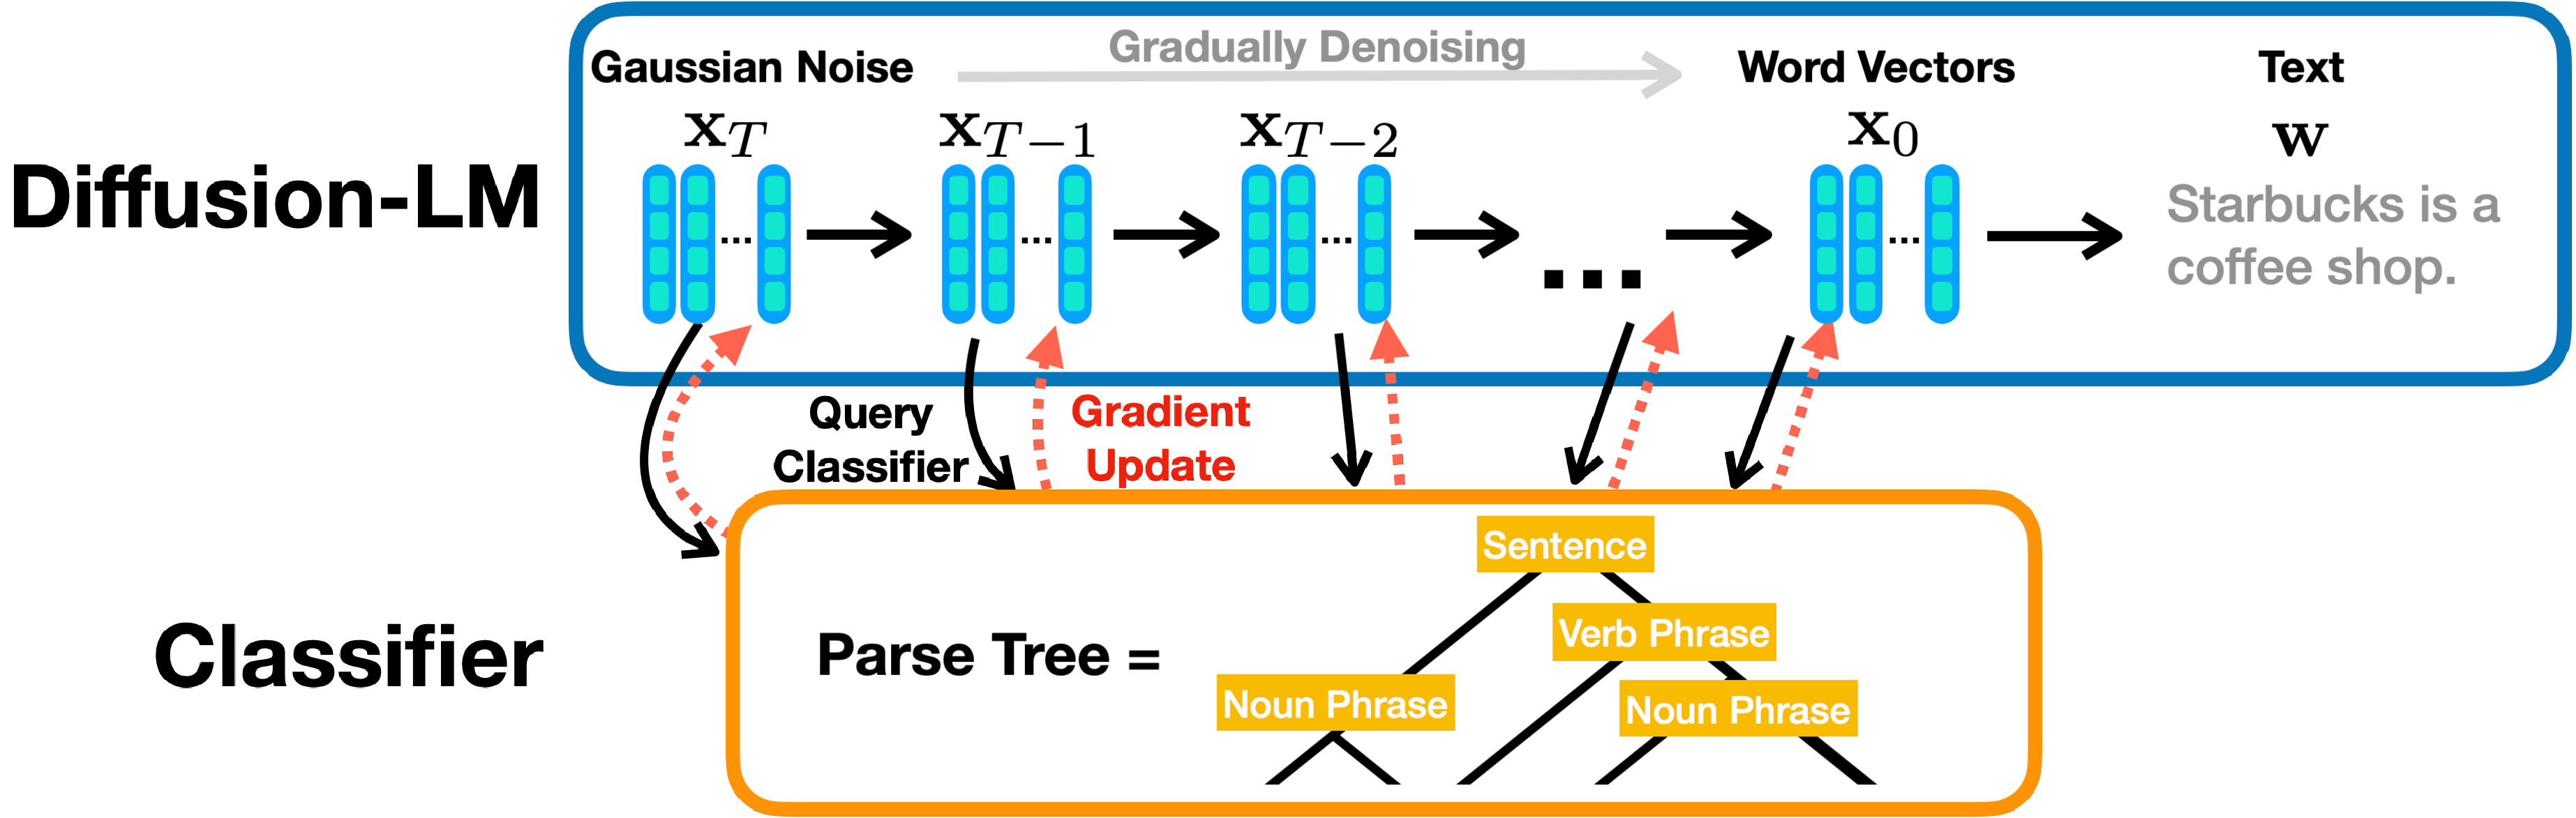
\includegraphics[width=0.8\textwidth]{fig/fig1_v2.pdf}
     \caption{\label{fig:1} Diffusion-LM은 가우시안 벡터 시퀀스를 단어 벡터로 반복적으로 디노이징하여, 노이즈 수준이 점점 낮아지는 중간 잠재변수 $\cx{T} \cdots \cx{0}$를 만든다. 제어 가능 생성에서는 이 연속 잠재변수에 반복적으로 경사 갱신을 수행하여, 유창성(Diffusion-LM이 매개변수화)과 제어 요구사항(분류기가 매개변수화)을 함께 최적화한다.
     \vspace{-5mm}
    }
\end{figure}


연속 디퓨전 모델은 비전·오디오 영역에서 큰 성공을 거두었지만 \cite{ho2020denoising,kong2020diffwave,ramesh2022hierarchical,dhariwal2021diffusion,chen2021wavegrad}, 텍스트는 본질적으로 이산(discrete)이라는 특성 때문에 텍스트에는 적용되지 못했다(\cref{sec:background}). 이 모델을 텍스트로 가져오려면 표준 디퓨전에 몇 가지 수정이 필요하다. 본 연구는 표준 디퓨전 과정에 임베딩(embedding) 단계와 반올림(rounding) 단계를 추가하고, 임베딩 학습을 위한 학습 목적함수를 설계하며, 반올림을 개선하기 위한 기법을 제안한다(\cref{sec:method}).
\cref{fig:1}처럼 경사 기반 방법으로 Diffusion-LM을 제어한다. 이 방법은 텍스트 생성 과정을 목표 구조·의미 제약을 만족하는 출력으로 유도할 수 있게 한다. 구체적으로, Diffusion-LM의 연속 잠재변수에 반복적으로 경사 갱신을 적용해 유창성과 제어 충족 사이의 균형을 맞춘다(\cref{ssec:control_text}).%

Diffusion-LM의 제어 능력을 시연하기 위해 의미 내용(semantic content) 같은 세밀 속성에서부터 파스 트리 같은 복잡 구조까지 6개 제어 목표를 다룬다.
본 방법은 기존 플러그앤플레이 방법의 성공률을 거의 두 배로 끌어올리고, 모든 분류기 유도(classifier-guided) 제어 과제에서 파인튜닝 오라클과 동등하거나 더 나은 성능을 보인다(\cref{ssec:control}).
또한 단일 제어 과제뿐 아니라, 여러 분류기 유도 제어를 조합해 원하는 의미 내용과 구문 구조를 동시에 만족하는 문장을 성공적으로 생성할 수 있음을 보인다(\cref{ssec:compose}).
끝으로, 길이 제어와 채우기(infilling)처럼 \emph{스팬(span)}에 닻을 둔 제어를 다룬다. Diffusion-LM은 이러한 제어 과제를 분류기 \emph{없이도} 수행할 수 있으며, 채우기 과제에서 기존 플러그앤플레이 방법을 큰 폭으로 능가하고, 처음부터 학습한 자기회귀 LM과 동등한 수준이다(\cref{ssec:infill}).

\section{관련 연구}
\label{sec:related_work}


\paragraph{텍스트를 위한 디퓨전 모델.}
디퓨전 모델 \cite{pmlr-v37-sohl-dickstein15}은 연속 데이터 영역에서 큰 성공을 거두며 \cite{ho2020denoising,nichol2021improved, kong2020diffwave, Mittal2021Music} 최첨단 표본 품질의 이미지·오디오를 만들어 냈다. 이산 데이터를 다루기 위해 기존 연구들은 \emph{이산(discrete)} 상태 공간에서의 텍스트 디퓨전을 연구했는데, 이는 이산 데이터에 손상(corruption) 과정을 정의한다(예: 각 토큰이 흡수 토큰 혹은 임의 토큰으로 확률적으로 손상됨) \cite{austin2021structured,hoogeboom2021argmax,hoogeboom2022autoregressive}.
본 논문은 텍스트를 위한 \emph{연속(continuous)} 디퓨전 모델에 초점을 맞추며, 우리가 아는 한 이 설정을 탐구한 최초의 연구이다.
이산 디퓨전 LM과 달리, 우리의 연속 디퓨전 LM은 연속 잠재 표현을 유도하며, 이는 제어 가능 생성에 효율적인 경사 기반 방법을 가능하게 한다.

\paragraph{자기회귀와 비자기회귀 LM.}
대부분의 대규모 사전학습(pre-training) LM은 좌→우 자기회귀이다(예: GPT-3 \cite{brown-et-al-gpt3}, PaLM \cite{Chowdhery2022PaLMSL}). 이러한 고정된 생성 순서는, 좌·우 문맥 모두에 대해 전역적으로 제어를 부과해야 하는 제어 가능 생성 환경에서 모델의 유연성을 제한한다. 예를 들어 채우기(infilling)는 우 문맥에 어휘 제약을 가하며, 구문 구조 제어는 좌·우 문맥을 모두 포함하는 전역 속성을 제어한다.
자기회귀 LM은 우 문맥에 직접 조건화할 수 없으므로, 이러한 과제에 대해 기존 연구는 특수 학습·디코딩 기법을 개발해 왔다 \cite{sha-2020-gradient,donahue-etal-2020-enabling,qin-etal-2020-back}.
예컨대 \citet{Qin-COLD}는 이산 LM 출력을 연속 변수로 완화하고, 우 문맥의 경사 정보를 역전파하는 디코딩 방법을 제안했다.
Diffusion-LM은 문장의 복잡하고 전역적인 속성을 보는 임의의 분류기에 조건화할 수 있다.
한편 기계 번역이나 음성-텍스트 변환을 위한 비자기회귀 LM도 개발되어 왔다 \cite{gu2018nonautoregressive,saharia2020latentalignments}.
그러나 이런 방법들은 출력의 엔트로피가 낮은 음성·번역 설정에 특화되어 있고, 일반 언어모델링에는 실패한다고 보고되었다 \cite{ren-etal-2020-study}.

\paragraph{플러그앤플레이 제어 가능 생성.}
플러그앤플레이 제어 가능 생성은 LM을 동결한 채, 잠재함수(예: 분류기)를 이용해 출력을 조정하는 것을 목표로 한다. 생성된 텍스트가 원하는 제어를 얼마나 잘 만족시키는지를 측정하는 확률적 잠재함수가 주어졌을 때, 생성 텍스트는 제어 충족(잠재함수로 측정)과 유창성(LM 확률로 측정) 모두에 대해 최적화되어야 한다.
자기회귀 LM 기반 플러그앤플레이 접근은 여러 가지가 있다.
FUDGE \cite{yang-klein-2021-fudge}는 부분 시퀀스에 대한 제어 충족 추정치로 매 토큰마다 LM 예측을 재가중한다.
GeDi \cite{KrauseGeDi2020}와 DExperts \cite{liu-etal-2021-dexperts}는 제어 과제용으로 파인튜닝/학습한 더 작은 LM을 사용해 매 토큰마다 LM 예측을 재가중한다.


우리 연구와 가장 가까운 것은 PPLM \cite{Dathathri2020Plug}이다. PPLM은 자기회귀 LM의 은닉 활성에 경사 상승(gradient ascent)을 적용해, 다음 토큰이 제어를 만족하고 유창성을 유지하도록 유도한다.
PPLM은 자기회귀 LM 기반이므로 좌→우로만 생성할 수 있다. 따라서 이전 생성 단계에서 발생한 오류를 복구·수정하지 못한다.
이들은 주제 같은 속성 제어에서는 성공했지만, \cref{ssec:control}에서 자기회귀 LM 기반의 이런 플러그앤플레이 방법이 구문 구조나 의미 내용 같은 더 복잡한 제어 과제에서는 실패함을 보인다. Diffusion-LM은 자신이 유도하는 연속 잠재변수 시퀀스에 분류기 유도 경사 갱신을 적용함으로써 플러그앤플레이 제어 가능 생성을 수행할 수 있음을 시연한다.




\newcommand{\xxtheta}{f_\theta}
\section{문제 설정과 배경}
\label{sec:background}

먼저 제어 가능 생성을 정의하고(\cref{ssec:control_setup}), 이어서 연속 디퓨전 모델을 검토한다(\cref{ssec:diffusion_setup}).

\subsection{텍스트의 생성 모델과 제어 가능 생성}
\label{ssec:control_setup}
텍스트 생성은 학습된 언어모델 $\plm (\ww)$에서 $\ww$를 표집하는 과제이다. 여기서 $\ww = [w_1 \cdots w_n]$은 이산 단어 시퀀스이고, $\plm (\ww)$는 단어 시퀀스에 대한 확률분포이다. 제어 가능 텍스트 생성은 조건부 분포 $p(\ww \mid \cc)$에서 $\ww$를 표집하는 과제로, $\cc$는 \emph{제어(control)} 변수이다. 구문 제어에서 $\cc$는 목표 구문 트리(\cref{fig:1})일 수 있고, 감성 제어에서 $\cc$는 원하는 감성 라벨일 수 있다. 제어 가능 생성의 목표는 제어 목표 $\cc$를 만족하는 $\ww$를 생성하는 것이다.

플러그앤플레이 제어 가능 생성 설정을 고려하자. 대량의 비라벨 텍스트로 학습된 언어모델 $\plm(\ww)$가 주어지고, 각 제어 과제마다 적은 양의 라벨 텍스트로 학습된 분류기 $p(\cc \mid \ww)$가 주어진다(예: 구문 제어의 경우 분류기는 확률적 파서이다). 목표는 이 두 모델을 활용하여 베이즈 규칙 $p(\ww \mid \cc) \propto \plm(\ww) \cdot p(\cc \mid \ww)$를 통해 사후 $p(\ww \mid \cc)$에서 근사적으로 표집하는 것이다. 여기서 $\plm(\ww)$는 $\ww$가 유창하도록, $p(\cc \mid \ww)$는 $\ww$가 제어를 충족하도록 유도한다.






\subsection{자기회귀 언어모델}
언어모델링의 표준 접근은 $\plm$을 좌→우로 자기회귀 분해하는 것이다: $\plm(\ww) = \plm(w_1) \prod_{i=2}^n \plm(x_i \mid x_{<i})$. 이 경우 텍스트 생성은 지금까지 생성된 부분 시퀀스에 조건화하여 다음 토큰을 반복적으로 예측하는 과제로 환원된다. 다음 토큰 예측 $\plm(x_i \mid x_{<i})$는 보통 Transformer 아키텍처 \cite{Vaswani2017Attn}로 매개변수화된다.

\subsection{연속 영역의 디퓨전 모델}
\label{ssec:diffusion_setup}

디퓨전 모델 \citep{ho2020denoising,nichol2021improved}은 데이터 $\cx{0} \in \mathbb{R}^d$를 마르코프 사슬(Markov chain) $\cx{T} \dots \cx{0}$로 모델링하는 잠재변수 모델이며, 각 변수가 $\mathbb{R}^d$에 속하고 $\cx{T}$는 가우시안이다. 디퓨전 모델은 잠재변수 시퀀스 $\cx{T:1}$을 점진적으로 디노이징하여 목표 데이터 분포의 표본을 근사한다(\cref{fig:graphical_model}). 초기 상태는 $p_\theta(\cx{T}) \approx \mathcal{N} (0, \mathbf{I})$이고, 각 디노이징 전이 $\cx{t} \rightarrow \cx{t-1}$는 모델 $\ptheta(\cx{t-1}\mid \cx{t}) = \mathcal{N}(\cx{t-1}; \mu_\theta(\cx{t}, t), \Sigma_\theta(\cx{t}, t))$로 매개변수화된다. 예를 들어 $\mu_\theta$, $\Sigma_\theta$는 U-Net이나 Transformer로 계산될 수 있다.


디퓨전 모델을 학습하기 위해, 중간 잠재변수 $\cx{1:T}$를 구성하는 정방향(forward) 과정을 정의한다. 정방향 과정은 데이터 $\cx{0}$에 가우시안 노이즈를 점진적으로 더하여, 디퓨전 단계 $T$에서 표본 $\cx{T}$가 근사적으로 가우시안이 되도록 한다. 각 전이 $\cx{t-1} \rightarrow \cx{t}$는 $q(\cx{t} \mid \cx{t-1}) = \mathcal{N} (\cx{t} ; \sqrt{1-\beta_t} \cx{t-1}, \beta_t \mathbf{I})$로 매개변수화되며, 하이퍼파라미터 $\beta_t$는 디퓨전 단계 $t$에서 더해지는 노이즈 양이다.
정방향 과정 $q$의 매개변수화는 학습 가능한 파라미터를 포함하지 않으며, 이를 통해 사전 정의된 정방향 과정 $q$로 노이즈 데이터를 만들고 모델이 그 과정을 역으로 풀어 데이터를 재구성하도록 학습하는 학습 목적함수를 정의할 수 있다.




\begin{figure}
    \centering
    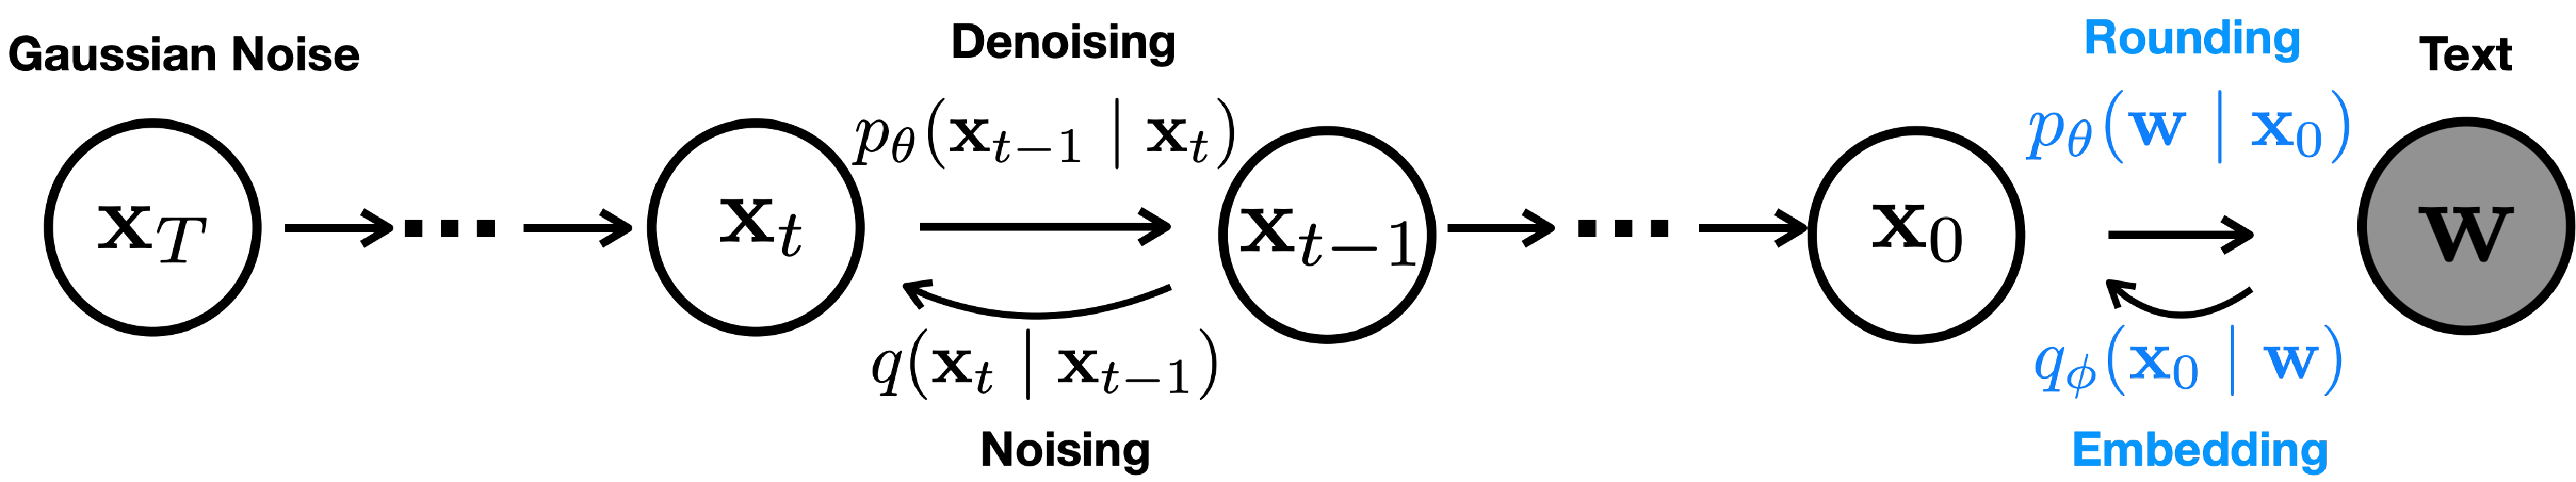
\includegraphics[width=0.8\textwidth]{fig/graphical_model_v2.pdf}
    \caption{\label{fig:graphical_model} 정방향·역방향 디퓨전 과정을 나타내는 그래픽 모델. 원래의 디퓨전 모델 \cite{ho2020denoising}에 더하여, 우리는 $\cx{0}$와 $\ww$ 사이에 마르코프 전이를 추가하고, 임베딩(\cref{ssec:embeddings})과 반올림(\cref{ssec:rounding}) 기법을 제안한다.}
    \vspace{-5mm}
\end{figure}

디퓨전 모델은 데이터의 주변 가능도 $\mathbb{E}_{\cx{0} \sim p_\text{data} }[\log p_\theta(\cx{0})]$를 최대화하도록 학습되며, 표준 목적함수는 $\log p_\theta(\cx{0})$의 변분 하한이다 \cite{pmlr-v37-sohl-dickstein15}.
\begin{equation}
\Lvlb (\cx{0}) = \mathop{\mathbb{E}}_{q(\cx{1:T} | \cx{0})} \left[\log \frac{q(\cx{T} | \cx{0})}{\ptheta(\cx{T})} + \sum_{t=2}^T \log \frac{q(\cx{t-1} | \cx{0},\cx{t})} {\ptheta(\cx{t-1} | \cx{t}) } - \log \ptheta( \cx{0} | \cx{1})\right].
\label{eqn:diffusion}
\end{equation}
하지만 이 목적함수는 불안정할 수 있고, 안정화에 많은 최적화 트릭을 필요로 한다 \cite{nichol2021improved}. 이 문제를 우회하기 위해 \citet{ho2020denoising}은 $\Lvlb$의 각 KL 발산 항을 전개·재가중하여 평균제곱오차 손실을 얻는 단순한 대리 목적함수를 고안했다(유도는 \cref{app:derive} 참조). 이를 다음과 같이 부른다.
\[\Lsimple (\cx{0}) = \sum_{t=1}^T \mathop{\mathbb{E}}_{q(\cx{t} \mid \cx{0})} || \mu_\theta(\cx{t}, t) - \hat{\mu}(\cx{t}, \cx{0}) ||^2,\]
여기서 $\hat{\mu}(\cx{t}, \cx{0})$는 닫힌 형식 가우시안인 사후 $q(\cx{t-1} | \cx{0},\cx{t})$의 평균이고, $\mu_\theta(\cx{t}, t)$는 신경망이 계산하는 $\ptheta(\cx{t-1} \mid \cx{t})$의 예측 평균이다.
$\Lsimple$은 더 이상 유효한 하한은 아니지만, 기존 연구에서 학습을 더 안정적으로 만들고 표본 품질을 향상시킨다고 경험적으로 보고되었다\footnote{우리의 $\Lsimple$ 정의는 \citet{ho2020denoising}과 다른 매개변수화를 사용한다. 우리는 제곱 손실을 $\mu_\theta(\cx{t}, t)$로 표현하지만 그들은 $\epsilon_\theta(\cx{t}, t)$로 표현한다.}.
Diffusion-LM에서도 학습 안정화와 표본 품질 향상을 위해 비슷한 단순화를 사용할 것이다(\cref{ssec:embeddings}).














\vspace{-2mm}
\section{Diffusion-LM: 연속 디퓨전 언어모델링}
\vspace{-2mm}
\label{sec:method}

Diffusion-LM 구성에는 표준 디퓨전 모델에 몇 가지 수정이 필요하다.
첫째, 이산 텍스트를 연속 공간으로 사상하는 임베딩 함수를 정의해야 한다. 이를 위해 임베딩을 학습하는 종단간 학습 목적함수를 제안한다(\cref{ssec:embeddings}).
둘째, 임베딩 공간의 벡터를 다시 단어로 사상하는 반올림 방법이 필요하다. 이를 위해 반올림을 돕는 학습 시·디코딩 시 방법을 제안한다(\cref{ssec:rounding}).








\vspace{-2mm}
\subsection{종단간 학습}
\label{ssec:embeddings}


이산 텍스트에 연속 디퓨전 모델을 적용하기 위해, 각 단어를 $\mathbb{R}^{d}$의 벡터로 사상하는 임베딩 함수 $\Emb(w_i)$를 정의한다. 길이 $n$ 시퀀스 $\ww$의 임베딩은 $\Emb(\ww) = [\Emb(w_1), \dots, \Emb(w_n)] \in \mathbb{R}^{nd}$로 정의한다.

식 \ref{eqn:diffusion}의 디퓨전 모델 학습 목적함수를 수정하여, 디퓨전 모델의 파라미터와 단어 임베딩을 함께 학습한다.
예비 실험에서 우리는 무작위 가우시안 임베딩과 사전학습 단어 임베딩 \cite{pennington-etal-2014-glove, radford2019language}을 모두 시도해 보았다. 이러한 고정 임베딩들은 종단간 학습에 비해 Diffusion-LM에 차선이라는 점을 발견했다\footnote{학습 가능한 임베딩이 제어·생성 과제에서 가장 좋지만, 어휘 단순체(simplex)로의 고정 임베딩이 홀드아웃 perplexity 최적화에는 도움이 됨을 확인했다. 본 연구의 초점은 perplexity가 아니라 생성 품질이므로 이 접근과 perplexity 결과의 논의는 \cref{app:simplex}로 미룬다.}.


그림 \ref{fig:graphical_model}처럼, 우리 접근은 정방향 과정에서 이산 단어 $\ww$로부터 $\cx{0}$로의 마르코프 전이를 추가하며, 이는 $\qphi(\cx{0} | \ww) = \mathcal{N} (\Emb(\ww), \sigma_0 I )$로 매개변수화된다. 역방향 과정에는 학습 가능한 반올림 단계를 추가하며, 이는 $\ptheta(\ww \mid \cx{0}) = \prod_{i=1}^n \ptheta(w_i \mid x_i)$로 매개변수화된다. 여기서 $\ptheta(w_i \mid x_i)$는 소프트맥스 분포이다. \cref{sec:background}에서 도입한 학습 목적함수는 이제 다음과 같아진다.
\begin{equation}
\begin{aligned}
\mathcal{L}^\text{e2e}_{\text{vlb}} (\ww) &= \mathop{\mathbb{E}}_{q_\phi(\cx{0} | \ww)}\left[\mathcal{L}_{\text{vlb}} (\cx{0}) + \log \qphi(\cx{0} | \ww) - \log \ptheta(\ww | \cx{0})]\right], \\
 \mathcal{L}^\text{e2e}_\text{simple} (\ww) &= \mathop{\mathbb{E}}_{\qphi(\cx{0:T} | \ww)} \left[\Lsimple(\cx{0}) + || \Emb(\ww) - \mu_\theta(\cx{1}, 1) ||^2  - \log \ptheta(\ww | \cx{0})\right].
\end{aligned}
\label{obj:e2e}
\end{equation}
\begin{wrapfigure}[11]{R}{0.5\textwidth}
\vspace{-10mm}
\centering
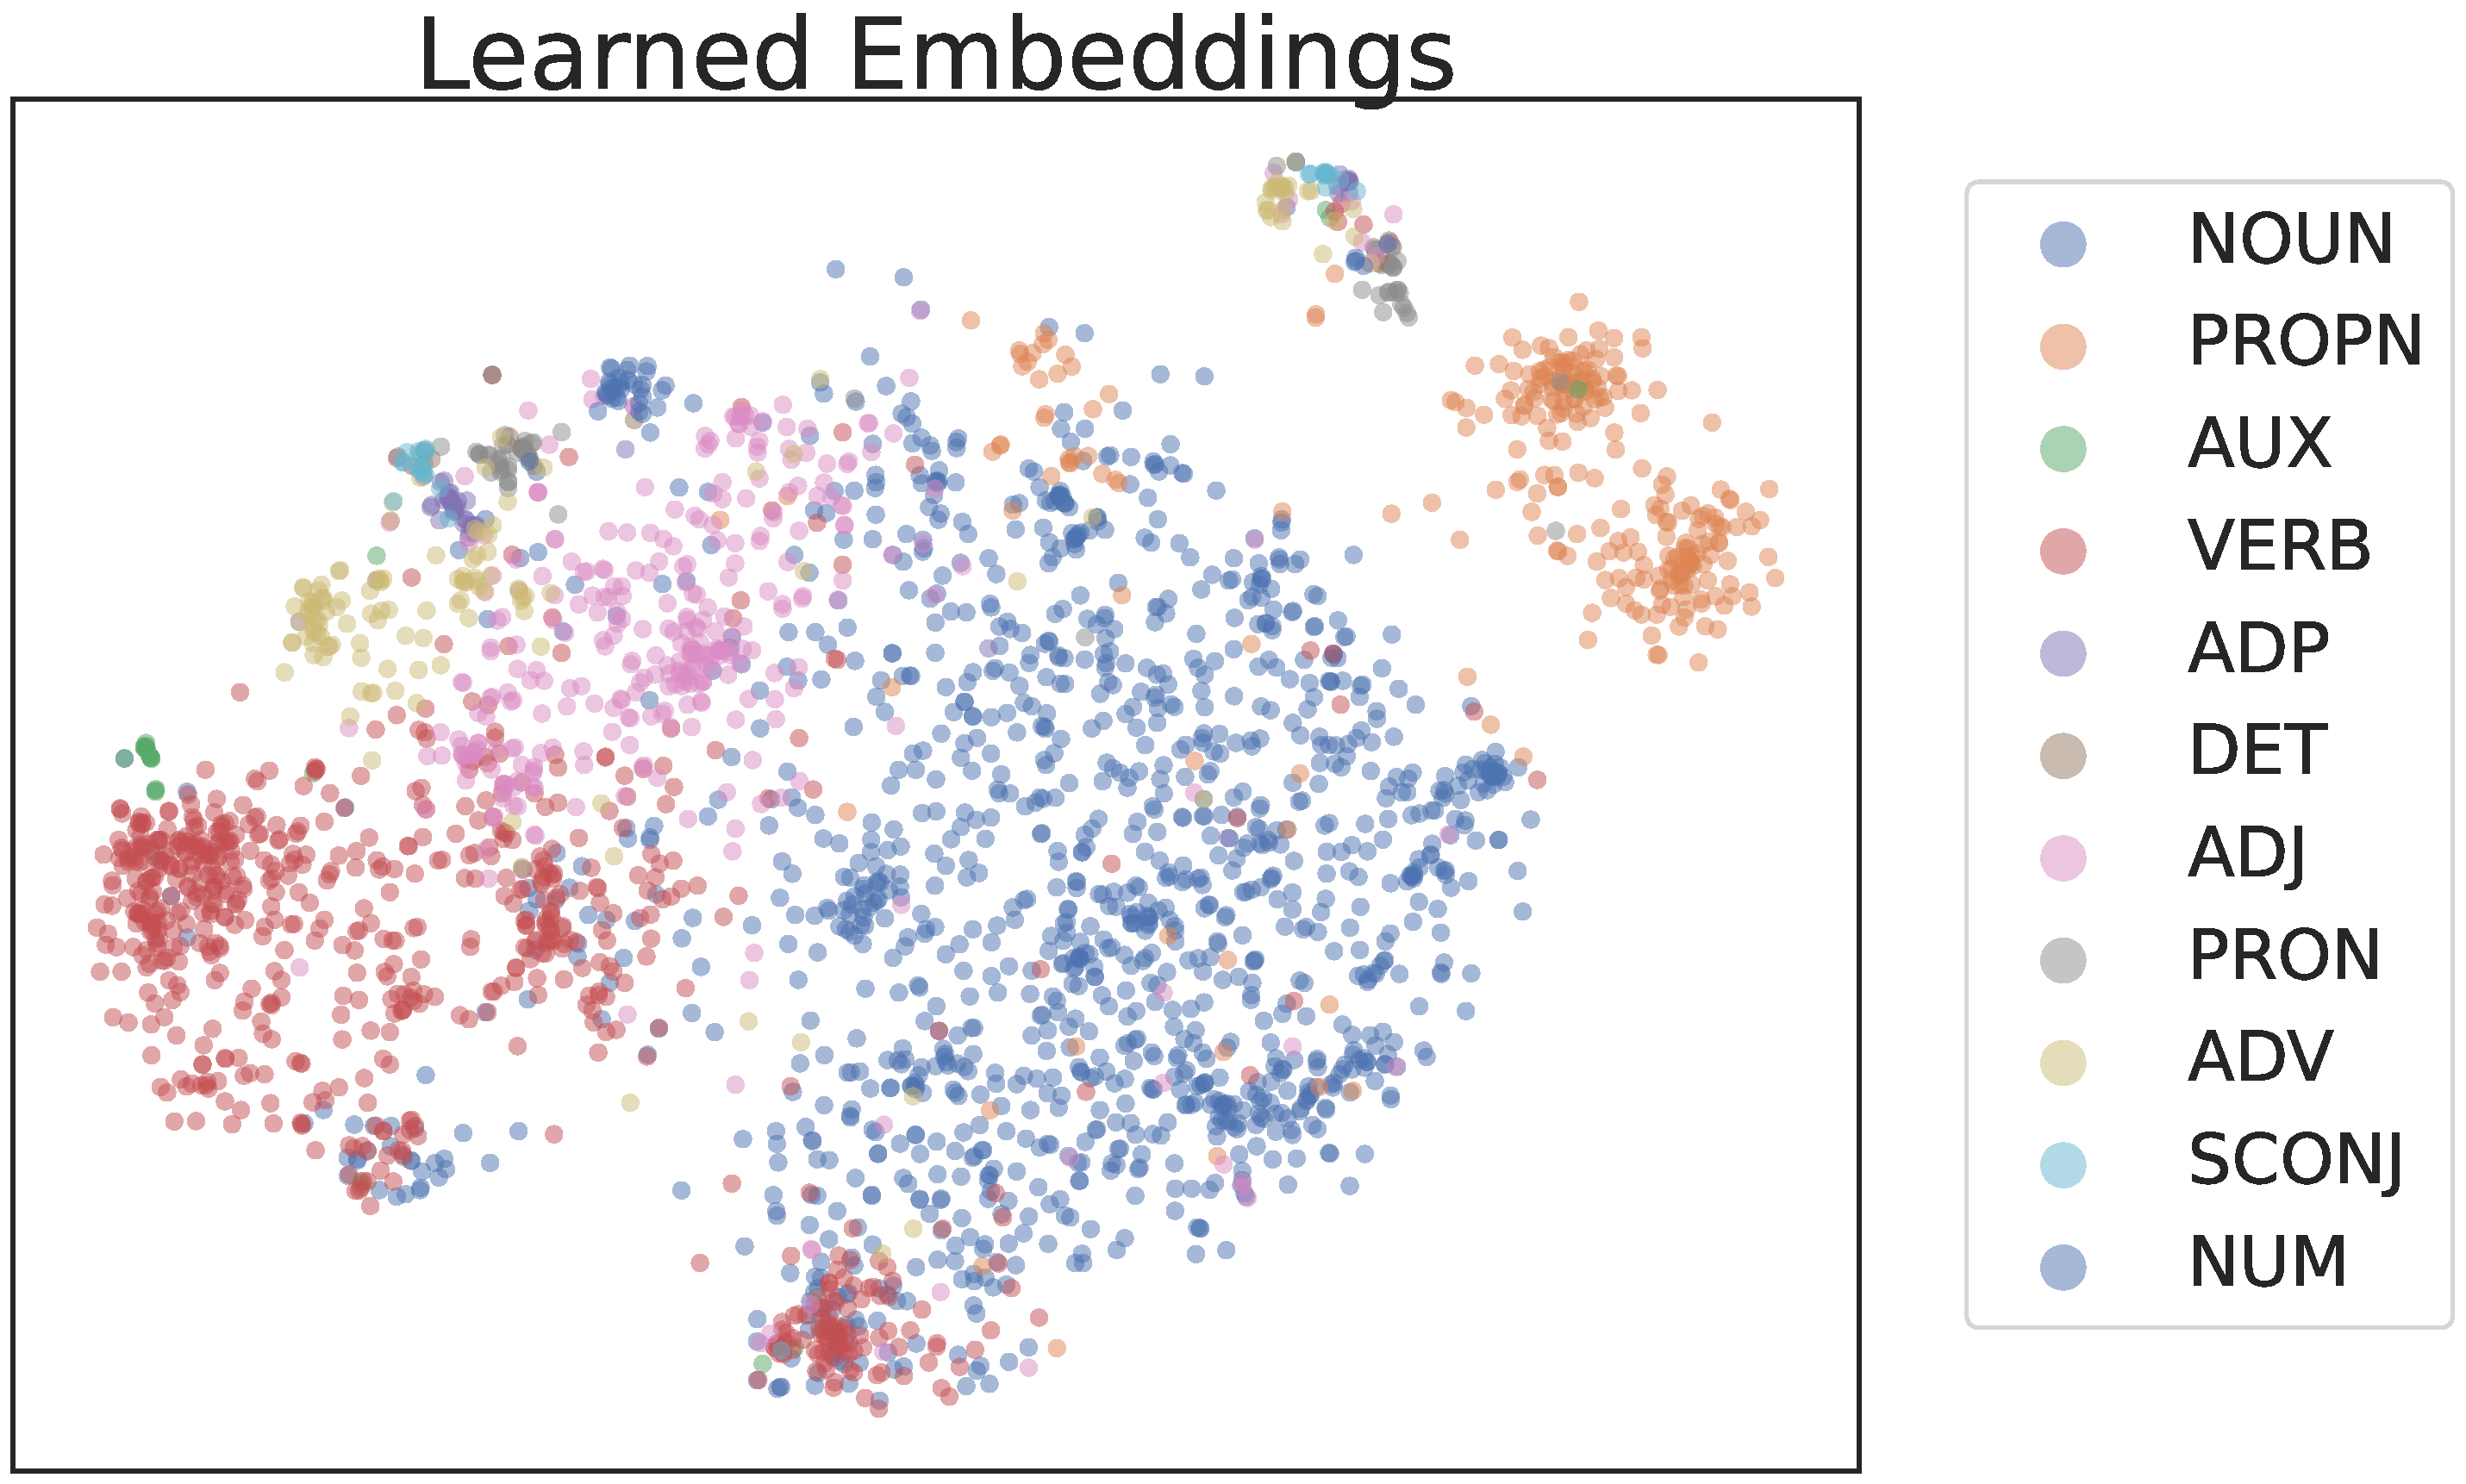
\includegraphics[width=\linewidth]{fig/embedding_128_v3.pdf}\caption{ \label{fig:emb} 학습된 단어 임베딩의 t-SNE \cite{vanDerMaaten2008} 도식. 각 단어는 그 품사로 색칠되어 있다. \looseness=-1 }
\end{wrapfigure}

$ \mathcal{L}^\text{e2e}_\text{simple} (\ww)$은 \cref{ssec:diffusion_setup}의 단순화를 따라 $\mathcal{L}^\text{e2e}_{\text{vlb}}(\ww)$로부터 유도하며, 자세한 유도는 \cref{app:derive}에 있다. 우리는 임베딩 함수를 학습하므로 이제 $q_\phi$가 학습 가능한 파라미터를 포함하며, 이 표집 단계를 통과하여 역전파하기 위해 재매개변수화 트릭 \citep{rezende2014stochastic, kingma2014auto}을 사용한다.
경험적으로 학습된 임베딩이 의미 있게 군집을 이룸을 확인했다. 같은 품사 태그(구문 역할)를 가진 단어들이 군집을 이루는 경향이 있으며, 이는 \cref{fig:emb}에 나타나 있다.



\subsection{반올림 오차 줄이기}
\label{ssec:rounding}


학습된 임베딩은 이산 텍스트에서 연속 $\cx{0}$로의 사상을 정의한다. 이제 예측된 $\cx{0}$를 다시 이산 텍스트로 반올림하는 역과정을 설명한다. 반올림은 위치마다 $\ptheta(\ww \mid \cx{0})= \prod_{i=1}^n \ptheta(w_i \mid x_i)$의 argmax에 따라 가장 확률이 높은 단어를 선택해 이루어진다. 이상적으로는 디노이징 단계가 $\cx{0}$를 어떤 단어의 임베딩 위에 정확히 놓이게 보장하기 때문에 argmax 반올림만으로 이산 텍스트로 사상하기에 충분해야 한다. 그러나 경험적으로 모델은 단일 단어에 정착하는 $\cx{0}$를 생성하지 못한다.



이 현상의 한 가지 설명은, 우리의 목적함수 \ref{obj:e2e}에서 $\Lsimple(\cx{0})$ 항이 $\cx{0}$의 구조를 모델링하는 데 충분히 무게를 두지 않는다는 것이다. $\Lsimple(\cx{0}) =\sum_{t=1}^T \mathbb{E}_{\cx{t}}|| \mu_\theta(\cx{t}, t) - \hat{\mu}(\cx{t}, \cx{0}) ||^2$의 정의를 떠올려 보자. 우리 모델 $\mu_\theta(\cx{t}, t)$는 디노이징 단계 $t$마다 $\ptheta(\cx{t-1}\mid \cx{t})$의 평균을 직접 예측한다.
이 목적함수에서 $\cx{0}$가 단일 단어 임베딩에 정착해야 한다는 제약은 $t$가 0에 가까운 항에서만 나타나며, 이러한 매개변수화는 그 항들을 강조하도록 목적함수를 신중하게 튜닝해야 함을 확인했다(\cref{app:ablation} 참고).


\newcommand{\Lsimplexx}{\mathcal{L}^\text{e2e}_{\cx{0}\text{-simple}}}
우리 접근은 $\Lsimple$을 재매개변수화하여 Diffusion-LM이 목적함수의 \emph{모든} 항에서 $\cx{0}$를 명시적으로 모델링하도록 강제한다. 구체적으로, $\cx{0}$로 매개변수화된 $\Lsimple$의 유사 형태인 $\Lsimplexx(\cx{0})=\sum_{t=1}^T \mathbb{E}_{\cx{t}} ||\xxtheta(\cx{t}, t) - \cx{0} ||^2$를 유도한다. 여기서 모델 $\xxtheta(\cx{t}, t)$는 $\cx{0}$를 직접 예측한다\footnote{$\cx{t-1}$의 분포는 정방향 과정 $\cx{t-1} = \sqrt{\alphabar} \cx{0} +\sqrt{1-\alphabar} \epsilon$로부터 닫힌 형식으로 얻을 수 있으므로, $\cx{0}$를 예측하는 것과 $\cx{t-1}$을 예측하는 것은 스케일링 상수까지 동치이다. 자세한 내용은 \cref{app:derive} 참고.}. 이는 신경망이 모든 항에서 $\cx{0}$를 예측하도록 강제하며, 이 목적함수로 학습한 모델은 $\cx{0}$가 단어 임베딩에 정확히 중심을 두어야 함을 빠르게 학습함을 확인했다.

위에서 모델 학습에 재매개변수화가 어떻게 도움이 되는지 설명했지만, 같은 직관을 디코딩 시에도 사용할 수 있는 기법이 있다. 이를 \emph{클램핑(clamping) 트릭}이라 부른다.
$\cx{0}$ 매개변수화 모델의 표준 생성 절차에서, 모델은 먼저 $\xxtheta(\cx{t}, t)$로 $\cx{0}$의 추정치를 계산한 뒤 이 추정치에 조건화하여 $\cx{t-1}$을 표집함으로써 $\cx{t}$를 $\cx{t-1}$로 디노이징한다: $\cx{t-1} = \sqrt{\alphabar} \xxtheta(\cx{t}, t) +\sqrt{1-\alphabar} \epsilon$, 여기서 $\alphabar_t = \prod_{s=0}^t (1-\beta_s)$, $\epsilon \sim \mathcal{N}(0,I)$\footnote{이는 모든 마르코프 전이가 가우시안이므로 닫힌 형식 가우시안이 되는 주변 분포 $q(\cx{t} \mid \cx{0})$로부터 따라 나온다.}. 클램핑 트릭에서는 모델이 추가로 예측 벡터 $\xxtheta(\cx{t}, t)$를 가장 가까운 단어 임베딩 시퀀스로 사상한다. 이제 표집 단계는 $\cx{t-1} = \sqrt{\alphabar}\cdot \Clamp(\xxtheta(\cx{t}, t)) +\sqrt{1-\alphabar} \epsilon$이 된다. 클램핑 트릭은 중간 디퓨전 단계의 예측 벡터가 단어에 정착하도록 강제하여 벡터 예측을 더 정확하게 만들고 반올림 오차를 줄인다.\footnote{직관적으로, $t$가 $T$에 가까운 초기 디퓨전 단계에 클램핑 트릭을 적용하는 것은 차선일 수 있다. 모델이 어떤 단어에 정착해야 할지 아직 결정하지 못했기 때문이다. 경험적으로 모든 디퓨전 단계에 클램핑 트릭을 적용해도 성능을 크게 해치지는 않는다. 다만 이 직관을 따르려면 클램핑 트릭의 시작 단계를 하이퍼파라미터로 둘 수도 있다.}


















\section{Diffusion-LM의 디코딩과 제어 가능 생성}
\label{sec:decode}
지금까지 Diffusion-LM을 설명했으며, 이제 제어 가능 텍스트 생성(\cref{ssec:control_text})과 디코딩(\cref{ssec:mbr1}) 문제를 다룬다.


\subsection{제어 가능 텍스트 생성}
\label{ssec:control_text}
이제 Diffusion-LM에서 플러그앤플레이 제어를 가능하게 하는 절차를 설명한다. \cref{ssec:control_setup}의 베이즈 정식화에서 영감을 얻되, 이산 텍스트에 직접 제어를 가하는 대신 Diffusion-LM이 정의하는 연속 잠재변수 시퀀스 $\cx{0:T}$에 제어를 가하고, 반올림 단계를 적용해 이 잠재변수들을 텍스트로 변환한다.

$\cx{0:T}$를 제어하는 일은 사후 $p(\cx{0:T} | \cc) = \prod_{t=1}^T p(\cx{t-1} \mid \cx{t}, \cc)$에서 디코딩하는 것과 동치이며, 이 결합 추론 문제를 각 디퓨전 단계의 제어 문제 시퀀스로 분해한다: $p(\cx{t-1} \mid \cx{t}, \cc) \propto p(\cx{t-1} \mid \cx{t}) \cdot p(\cc \mid \cx{t-1}, \cx{t})$.
이를 디퓨전 제어에 대한 기존 연구 \cite{song2021scorebased}의 조건부 독립 가정을 통해 $p(\cc \mid \cx{t-1}, \cx{t})=p(\cc \mid \cx{t-1})$로 더 단순화한다. 따라서 $t$번째 단계에서 우리는 $\cx{t-1}$에 대해 경사 갱신을 수행한다.
\begin{align*}
    \nabla_{\cx{t-1}} \log p(\cx{t-1} \mid \cx{t}, \cc) = \nabla_{\cx{t-1}} \log p(\cx{t-1} \mid \cx{t}) + \nabla_{\cx{t-1}}  \log  p(\cc \mid \cx{t-1}),
\end{align*}
여기서 $\log p(\cx{t-1} \mid \cx{t})$와 $\log p(\cc \mid \cx{t-1})$ 모두 미분 가능하다. 첫 항은 Diffusion-LM이 매개변수화하고, 두 번째 항은 신경망 분류기가 매개변수화한다.


이미지 영역의 연구 \cite{dhariwal2021diffusion,song2021scorebased}와 마찬가지로, 디퓨전 잠재변수에 대해 분류기를 학습하고 잠재 공간 $\cx{t-1}$에서 경사 갱신을 수행하여 제어를 충족하는 방향으로 유도한다. 이 이미지 디퓨전 연구들은 디퓨전 단계마다 $\nabla_{ \cx{t-1}} \log  p(\cc \mid \cx{t-1})$ 방향으로 한 번의 경사 단계를 취한다. 텍스트에서 성능을 높이고 디코딩을 가속하기 위해, 두 가지 핵심 변경을 도입한다: 유창성 정규화와 다중 경사 단계. \looseness=-1




유창한 텍스트를 생성하기 위해, \emph{유창성 정규화}가 포함된 제어 목적함수에 경사 갱신을 적용한다: $ \lambda \log p(\cx{t-1} \mid \cx{t}) + \log p(\cc \mid \cx{t-1})$. 여기서 $\lambda$는 유창성(첫 항)과 제어(둘째 항)를 절충하는 하이퍼파라미터이다. 디퓨전을 위한 기존 제어 가능 생성 방법은 목적함수에 $\lambda \log p(\cx{t-1} \mid \cx{t})$ 항을 포함하지 않지만, 이 항이 유창한 텍스트 생성에 결정적임을 확인했다. 이로 인한 제어 가능 생성 과정은 $p(\cx{t-1} \mid \cx{t}, \cc)$의 최대화와 표집 사이를 균형 짓는 확률적 디코딩 방법으로 볼 수 있으며, 이는 뉴클리어스 샘플링(nucleus sampling) \cite{Holtzman2020Nucleus}이나 낮은 온도(temperature) 샘플링 같은 텍스트 생성 기법과 비슷하다. 제어 품질을 높이기 위해 디퓨전 단계마다 다중 경사 단계를 취한다. 디퓨전 단계마다 Adagrad \footnote{Adagrad 대신 SGD를 사용하는 어블레이션도 시도했지만, Adagrad가 하이퍼파라미터 튜닝에 훨씬 덜 민감함을 확인했다.} \cite{Duchi2010AdaptiveSM} 갱신을 3 단계 수행한다. 늘어난 계산 비용을 완화하기 위해 디퓨전 단계 수를 2000에서 200으로 다운샘플링하면, 표본 품질을 크게 해치지 않으면서 제어 가능 생성 알고리즘이 가속된다.


\subsection{최소 베이즈 위험 디코딩}
\label{ssec:mbr1}
기계 번역이나 문장 채우기처럼 많은 조건부 텍스트 생성 과제는 \emph{단일} 고품질 출력 시퀀스를 요구한다.
이 환경에서, Diffusion-LM에서 표집한 샘플 집합 $\mathcal{S}$를 모은 뒤 손실함수 $\mathcal{L}$(예: 음의 BLEU 점수) 하에서 기대 위험을 최소화하는 샘플을 선택하는 최소 베이즈 위험(Minimum Bayes Risk, MBR) 디코딩 \cite{kumar-byrne-2004-minimum}을 적용한다: $\hat{\ww} = \argmin_{\ww \in S} \sum_{\ww' \in S} \frac{1}{|S|}\mathcal{L}(\ww, \ww')$. 저품질 샘플은 나머지 샘플들과 다르고 손실함수에 의해 패널티를 받기 때문에, MBR 디코딩이 흔히 고품질 출력을 반환함을 확인했다.







\newcommand{\Length}{Length\xspace}
\newcommand{\Spans}{Syntax Spans\xspace} 
\newcommand{\POS}{Parts-of-speech\xspace}
\newcommand{\Syntax}{Syntax Tree\xspace} 
\newcommand{\Content}{Semantic Content\xspace} 

\section{실험 설정}
위에서 설명한 학습(\cref{sec:method})과 디코딩(\cref{sec:decode})의 개선을 적용해, 두 가지 언어모델링 과제에 대해 Diffusion-LM을 학습한다. 그런 다음 제어 가능 생성 방법을 5개의 분류기 유도 제어 과제에 적용하고, 분류기 비의존 제어 과제(즉, 채우기)에는 MBR 디코딩을 적용한다.

\label{sec:setup}
\subsection{데이터셋과 하이퍼파라미터}
Diffusion-LM은 E2E \cite{novikova-etal-2017-e2e}와 ROCStories \cite{mostafazadeh-etal-2016-corpus} 두 데이터셋으로 학습한다. E2E 데이터셋은 음식 종류, 가격, 고객 평점 등 8개 필드로 라벨링된 5만 건의 식당 리뷰로 구성된다.
ROCStories 데이터셋은 5문장짜리 스토리 9만 8천 건으로 구성되며, 일상 사건들 사이의 풍부한 인과·시간적 상식 관계를 담고 있다.
이 데이터셋은 E2E보다 모델링이 더 어렵다. 스토리들이 1만 1천 단어 규모의 더 큰 어휘와 더 다양한 의미 내용을 포함하기 때문이다.


Diffusion-LM은 8천만 파라미터의 트랜스포머(Transformer) \cite{Vaswani2017Attn} 아키텍처를 기반으로 하며, 시퀀스 길이 $n=64$, 디퓨전 단계 $T=2000$, 그리고 제곱근 노이즈 스케줄(상세는 \cref{app:noise} 참고)을 사용한다. 임베딩 차원은 하이퍼파라미터로 두어 E2E에는 $d=16$, ROCStories에는 $d=128$로 설정한다. 하이퍼파라미터의 자세한 내용은 \cref{app:hyperparam}을 보라.
디코딩 시에는 E2E의 경우 200 디퓨전 단계로 다운샘플링하고, ROCStories는 2000 단계를 유지한다. Diffusion-LM을 200단계로 디코딩해도 자기회귀 LM 디코딩보다 7배 느리다. 제어 가능 생성에서, Diffusion-LM 기반의 본 방법은 FUDGE보다 1.5배 느리지만 PPLM보다는 60배 빠르다.


\subsection{제어 과제}
\label{ssec:control_gen_setup}

\begin{table*}
    \centering
    \resizebox{0.95\linewidth}{!}{
    \begin{tabular}{lp{13cm}}
\toprule
input (\Content) & food : Japanese\\
output text & Browns Cambridge is good for Japanese food and also children friendly near The Sorrento . \\
 \midrule
input (\POS) & PROPN AUX DET ADJ NOUN NOUN VERB ADP DET NOUN ADP DET NOUN PUNCT\\
output text & Zizzi is a local coffee shop located on the outskirts of the city . \\
\midrule
input (\Syntax)  & (TOP (S (NP (*) (*) (*)) (VP (*) (NP (NP (*) (*))))))\\
output text & The Twenty Two has great food \\
\midrule
input (\Spans) & (7, 10, VP) \\ 
output text & Wildwood pub serves multicultural dishes and is ranked 3 stars\\ 
\midrule
input (\Length) & 14 \\
output text & Browns Cambridge offers Japanese food located near The Sorrento in the city centre . \\
\midrule
input (left context) & My dog loved tennis balls.\\ 
input (right context)  & My dog had stolen every one and put it under there.\\ 
output text & One day, I found all of my lost tennis balls underneath the bed. \\
\bottomrule
\end{tabular}}
\caption{\label{app:example} 각 제어 과제별 입력 제어와 출력 텍스트의 예시(원문 그대로 영문 표기). \emph{역자 주: \Content/\POS/\Syntax/\Spans/\Length 등 매크로 라벨은 영문 그대로 유지.}}
\end{table*}

\cref{app:example}에 나타낸 6개의 제어 과제를 다룬다. 처음 4개 과제는 분류기에 의존하며, 마지막 2개 과제는 분류기 비의존이다\footnote{길이 제어는 우리의 Diffusion-LM 기반 방법에서는 분류기 비의존이지만, 다른 방법에서는 여전히 분류기를 필요로 한다.}.
각 제어 과제(예: 의미 내용)에 대해 검증 분할에서 200개의 제어 목표 $\cc$(예: rating=5 star)를 표집하고, 각 제어 목표마다 50개의 샘플을 생성한다.
생성 텍스트의 유창성을 평가하기 위해 기존 연구 \cite{yang-klein-2021-fudge, Dathathri2020Plug}를 따라 생성 텍스트를 교사(teacher) LM(즉, 신중하게 파인튜닝된 GPT-2 모델)에 입력하고, 교사 LM 하에서의 생성 텍스트 perplexity를 보고한다. 이 지표를 lm-score(약어 lm)라 부르며, 값이 낮을수록 표본 품질이 좋다.\footnote{기존 연구 \cite{yang-klein-2021-fudge, Dathathri2020Plug}는 교사 LM으로 GPT \cite{Radford2018ImprovingLU}를 사용하지만, 우리의 기준 자기회귀 LM과 Diffusion-LM 모두 UNK 토큰을 생성할 수 있고 GPT의 사전학습 어휘에는 UNK가 없으므로, 우리는 파인튜닝된 GPT-2 모델을 사용한다.}
각 제어 과제별 성공 지표는 다음과 같이 정의한다.

\textbf{\Content.} 필드(예: rating)와 값(예: 5 star)이 주어졌을 때, field=value를 포함하는 문장을 생성하고, `value'의 정확 일치(exact match)로 성공률을 보고한다.




\textbf{\POS.} 품사(part-of-speech, POS) 태그 시퀀스(예: \textit{Pronoun Verb Determiner Noun})가 주어졌을 때, 같은 길이의 단어 시퀀스를 생성하되 오라클 POS 태거로 측정한 품사가 목표와 일치해야 한다(예: \textit{I ate an apple}). 단어 수준 정확 일치로 성공을 정량화한다.


\textbf{\Syntax.} 목표 구문 파스 트리가 주어졌을 때(\cref{fig:1} 참고), 그 파스에 일치하는 구문 파스를 가지는 텍스트를 생성한다. 평가에서는 생성 텍스트를 기성 파서 \cite{kitaev-klein-2018-constituency}로 파싱한 뒤 F1 점수를 보고한다.


\textbf{\Spans.} %
목표 (스팬, 구문 범주) 쌍이 주어졌을 때, 스팬 $[i,j]$ 위의 파스 트리가 목표 구문 범주(예: 전치사구(prepositional phrase))와 일치하는 텍스트를 생성한다. 정확히 일치하는 스팬의 비율로 성공을 정량화한다.


\textbf{\Length.} 목표 길이 $10, \dots, 40$이 주어졌을 때, 목표의 $\pm 2$ 이내 길이의 시퀀스를 생성한다. Diffusion-LM에서는 이를 분류기 비의존 제어 과제로 다룬다.

\textbf{채우기(Infilling).} aNLG 데이터셋 \cite{bhagavatula2020abductive}에서 좌 문맥($O_1$)과 우 문맥($O_2$)이 주어지며, 목표는 $O_1$과 $O_2$를 논리적으로 연결하는 문장을 생성하는 것이다. 평가에서는 Genie 리더보드 \cite{Khashabi2021GENIEAL}의 자동 평가와 사람 평가 결과를 함께 보고한다.


\subsection{분류기 유도 제어 기준선}

처음 5개 제어 과제에 대해 PPLM, FUDGE, 파인튜닝 오라클과 본 방법을 비교한다. PPLM과 FUDGE는 자기회귀 LM에 기반한 플러그앤플레이 제어 가능 생성 접근으로, 우리는 GPT-2 small 아키텍처 \cite{radford2019language}를 사용해 처음부터 학습한다.


\textbf{PPLM \cite{Dathathri2020Plug}.} 이 방법은 LM 활성에 경사 상승을 적용해 분류기 확률과 언어모델 확률을 동시에 높이며, 단순 속성 제어에 성공해 왔다. 의미 내용 제어에는 PPLM을 적용하지만, 위치 정보가 필요한 나머지 4개 과제에는 적용하지 않는다. PPLM의 분류기는 위치 정보를 갖지 않기 때문이다.

\textbf{FUDGE \cite{yang-klein-2021-fudge}.} 각 제어 과제에 대해 FUDGE는 접두 시퀀스를 입력으로 받아 완전한 시퀀스가 제약을 만족할지 예측하는 미래 판별기(future discriminator)를 필요로 한다. 디코딩 시 FUDGE는 판별기 점수로 LM 예측을 재가중한다.

\textbf{FT.} 각 제어 과제에 대해 (제어, 텍스트) 쌍으로 GPT-2를 파인튜닝하여, 플러그앤플레이가 아닌 \emph{오라클} 조건부 언어모델을 얻는다.
파인튜닝 모델의 샘플링(temperature 1.0)과 빔 탐색(beam size 4) 출력을 모두 보고하며, 각각 FT-sample, FT-search로 표기한다.

\subsection{채우기 기준선}

채우기 과제에 대해 기존 연구의 특화된 기준선 3개와 비교한다.

\textbf{DELOREAN \cite{qin-etal-2020-back}.} 이 방법은 좌→우 자기회귀 LM의 출력 공간을 연속적으로 완화한 뒤, 연속 공간에서 반복적으로 경사 갱신을 수행해 우 문맥과의 유창한 연결을 강제한다. 그 결과 얻은 연속 벡터를 다시 텍스트로 반올림한다.

\textbf{COLD \cite{Qin-COLD}.} COLD는 좌→우와 우→좌 LM에서 오는 유창성, 그리고 어휘 중첩에서 오는 일관성 제약을 포함하는 에너지 기반 모델을 정의한다. 이 에너지 기반 모델에서 연속 벡터를 표집해 텍스트로 반올림한다.


\textbf{AR-infilling.} 문장 채우기 과제 \cite{donahue-etal-2020-enabling}를 위해 자기회귀 LM을 처음부터 학습한다. Diffusion-LM 학습과 마찬가지로 ROCStories 데이터셋으로 학습하지만, 문장을 $(O_1, O_\text{middle} , O_2)$에서 $(O_1, O_2, O_\text{middle})$로 재배열하는 전처리를 적용한다. 평가 시에는 $O_1, O_2$를 입력으로 주면 모델이 가운데 문장을 생성한다.










\section{주요 결과}
E2E와 ROCStories 데이터셋에서 Diffusion-LM을 학습한다.
음의 로그가능도(negative log-likelihood, NLL, 낮을수록 좋음) 기준으로, Diffusion-LM NLL의 변분 상한\footnote{Diffusion-LM의 정확한 로그가능도는 다루기 어렵기 때문에 하한 $\mathcal{L}^\text{e2e}_{\text{vlb}}$를 보고한다.}은 동등한 자기회귀 Transformer 모델보다 떨어진다(E2E: 2.28 vs. 1.77, ROCStories: 3.88 vs. 3.05). 다만 모델·데이터셋 크기를 키우면 격차가 일부 메워진다(ROCStories에서 3.88 $\xrightarrow{}$ 3.10).
최고의 로그가능도를 얻으려면 \cref{sec:method}에서 몇 가지 수정이 필요하며, 이를 \cref{app:simplex}에서 자세히 설명하고 로그가능도 결과를 함께 제시한다.
가능도는 떨어지지만, Diffusion-LM 기반 제어 가능 생성은 자기회귀 LM 기반 시스템보다 훨씬 나은 출력을 만들어 낸다. 이는 \cref{ssec:control}, \cref{ssec:compose}, \cref{ssec:infill}에서 보인다.

\newcommand{\fluency}{lm $\downarrow$}
\newcommand{\success}{ctrl $\uparrow$}



\subsection{분류기 유도 제어 가능 텍스트 생성 결과}
\label{ssec:control}
\begin{table*}
\centering
\resizebox{1.0\columnwidth}{!}{
\begin{tabular}{lcc|cc|cc|cc|cc}
\toprule
          & \multicolumn{2}{c|}{\Content} & \multicolumn{2}{c|}{\POS} & \multicolumn{2}{c|}{\Syntax} & \multicolumn{2}{c|}{\Spans} & \multicolumn{2}{c}{\Length}  \\
& \success        & \fluency       & \success     & \fluency    & \success     & \fluency     & \success     & \fluency    &  \success     & \fluency    \\ \hline
PPLM      &    9.9   & 5.32  &  - & - & - & - & - & - & - &  - \\
FUDGE     & 69.9 & 2.83  & 27.0  & 7.96     & 17.9   & \textbf{3.39} & 54.2 & 4.03 & 46.9  & 3.11   \\
Diffusion-LM & \textbf{81.2}  & \textbf{2.55}  &\textbf{90.0} & \textbf{5.16 }   & \textbf{86.0}    & 3.71 & \textbf{93.8} & \textbf{2.53}  & \textbf{99.9} & \textbf{2.16}   \\
\midrule
 FT-sample  & 72.5  & 2.87  & 89.5 & 4.72    & 64.8   & 5.72 & 26.3 & 2.88  & 98.1 & 3.84\\
FT-search  & 89.9  & 1.78  & 93.0 & 3.31    & 76.4   & 3.24 & 54.4 & 2.19  & 100.0 & 1.83\\
\bottomrule
\end{tabular}
}
\caption{\label{tab:control} Diffusion-LM은 5개 제어 과제 전반에서 높은 성공률(\success)과 좋은 유창성(\fluency)을 달성하여 PPLM·FUDGE 기준선을 능가한다. 본 방법은 구문 파스 트리·스팬 제어에서는 파인튜닝 오라클(FT)보다도 더 좋다.}
\end{table*}
\cref{tab:control}이 보여 주듯, Diffusion-LM은 모든 분류기 유도 제어 과제에서 높은 성공률과 유창성을 달성한다. 5개 과제 전반에서 PPLM과 FUDGE 기준선을 큰 폭으로 능가한다. 놀랍게도, 구문 파스 트리·스팬 제어에서는 파인튜닝 오라클까지 능가하고, 나머지 3개 과제에서도 비슷한 성능을 낸다.

구문 파스 트리와 스팬 제어는 파인튜닝에도 까다로운 과제이다. 파스 트리에 조건화하려면 파스의 중첩 구조를 추론해야 하고, 스팬에 조건화하려면 올바른 구성요소가 목표 위치에 나타나도록 사전(lookahead) 계획이 필요하기 때문이다.

PPLM은 의미 내용 제어에서 실패하는데, 이는 PPLM이 조립이 단순한 속성(coarse-grained attribute) 제어용으로 설계되었고, 식당 리뷰가 ``Starbucks''에 대한 언급을 포함하도록 강제하는 것 같은 보다 표적화된 과제에는 적합하지 않기 때문이라고 추측한다.


FUDGE는 의미 내용 제어에서는 잘 동작하지만 나머지 네 과제에서는 그렇지 못하다. 구조화된 출력(\POS, \Syntax)을 제어하기가 FUDGE에는 어려운데, 접두 어디에서든 한 번의 실수가 있으면 판별기가 모든 연장(continuation)에 낮은 확률을 부여하기 때문이다. 계획이 필요한 다른 제어 과제(\Length, \Spans)에서는 미래 판별기를 학습하기 어렵다. 사전 계획을 암묵적으로 수행해야 하기 때문이다.

Diffusion-LM의 비자기회귀 특성 덕분에 정밀한 미래 계획이 필요한 과제(\Spans, \Length)를 쉽게 풀 수 있다. 전역 구조가 관여하는 복잡 제어(\POS, \Syntax)에서도 잘 작동하는 이유는, 거친-세밀 표현이 분류기로 하여금 시퀀스 전체에 대한 제어($t=T$ 근방)와 개별 토큰에 대한 제어($t=0$ 근방)를 모두 행사할 수 있게 하기 때문이라고 본다.

\paragraph{정성적 결과.}
\Cref{app:qualitative-syntax}는 \Syntax 제어의 샘플을 보여 준다. 우리 방법과 파인튜닝은 대체로 제어를 만족하는 유창한 문장을 만들어 내지만, FUDGE는 처음 몇 단어 이후로 제약에서 이탈한다.
우리 방법과 파인튜닝의 핵심 차이는, Diffusion-LM은 실패한 스팬을 보정하고 이후 스팬은 목표에 일치시킬 수 있다는 점이다. 첫 번째 예에서 생성된 스팬(``Family friendly Indian food'')은 목표보다 단어가 1개 많아 틀렸다. 다행히 Diffusion-LM이 접속사를 빼는 식으로 조정하기 때문에 이 오류가 이후 스팬으로 전파되지 않는다. 두 번째 예에서 FT 모델이 생성한 실패 스팬(``The Mill'')은 단어가 1개 부족하다. 그러나 FT 모델은 접미부에서 조정에 실패해 접미부 전체에 정렬 오류가 누적된다.
\begin{table*}
    \centering
    \resizebox{0.95\linewidth}{!}{
    \begin{tabular}{lp{14cm}}
    \toprule
    Syntactic Parse & ( S ( S ( NP * ) ( VP * ( NP ( NP * * ) ( VP * \tgtspan{( NP ( ADJP * * ) * )} ) ) ) ) * ( S ( NP * * * ) ( VP * ( ADJP ( ADJP * ) ) ) ) )\\
    \midrule
FUDGE &  \errorspan{Zizzi is a cheap restaurant . \textbf{[incomplete]}} \\
Diffusion-LM &   Zizzi is a pub providing \errorspan{\textbf{family friendly Indian food}} Its customer rating is low \\
FT &  Cocum is a Pub serving \corrspan{\textbf{moderately priced meals}} and the customer rating is high \\
\toprule
     Syntactic Parse  &  ( S ( S ( VP * ( PP * ( NP * * ) ) ) ) * \tgtspan{( NP * * * )} ( VP * ( NP ( NP * * ) ( SBAR ( WHNP * ) ( S ( VP * ( NP * * ) ) ) ) ) ) * ) \\
\midrule
FUDGE &   \errorspan{In the city near The Portland Arms is a coffee and fast food place named The Cricketers which is not family - friendly with a customer rating of 5 out of 5 .} \\
Diffusion-LM &  Located on the riverside , \textbf{\corrspan{The Rice Boat}} is a restaurant that serves Indian food . \\
FT &  Located near The Sorrento, \errorspan{\textbf{The Mill} is a pub that serves Indian cuisine.} \\
    \bottomrule
    \end{tabular}}
\caption{\label{app:qualitative-syntax}  \Syntax 제어의 정성적 예시. 구문 파스 트리는 구성요소를 나타내는 중첩 괄호로 선형화되어 있으며, 표준 PTB 구문 범주를 사용한다. 각 스팬 안의 토큰은 *로 표기된다. 실패한 스팬은 \errorspan{빨강}, \cref{ssec:control}에서 논의하는 관심 스팬은 \textbf{굵게} 표시한다. (입출력 예시는 영문 그대로 둔다.)}
\end{table*}







\subsection{제어의 조합}
\label{ssec:compose}
\begin{table*}
    \centering
    \resizebox{0.85\linewidth}{!}{
\begin{tabular}{lccc|ccc}
\toprule

          & \multicolumn{3}{c|}{\Content + \Syntax} & \multicolumn{3}{c}{\Content + \POS }  \\
& semantic \success     & syntax \success      & \fluency       & semantic \success    & POS \success     & \fluency    \\ \hline
FUDGE           &  61.7     & 15.4   & 3.52 & 64.5 & 24.1 & 3.52\\
Diffusion-LM    &  \textbf{69.8}     & \textbf{74.8}  & 5.92 &  \textbf{63.7} & \textbf{69.1} & 3.46\\

\midrule

FT-PoE              &  61.7     & 29.2  & \textbf{2.77} &  29.4 & 10.5 & \textbf{2.97} \\
\bottomrule
\end{tabular}
 }
\caption{\label{tab:compose} 본 실험에서는 의미 제어와 구문 제어를 조합한다. Diffusion-LM은 유창성(\fluency)을 다소 양보하며 더 높은 성공률(\success)을 달성한다. 본 방법은 제어 성공률에서 FUDGE와 FT-PoE(두 파인튜닝 모델의 전문가 곱(product of experts)) 모두를 능가하며, 특히 구조화된 구문 제어(즉, 구문 파스 트리와 POS)에서 격차가 크다.
}
\end{table*}


플러그앤플레이 제어 가능 생성의 고유한 능력 중 하나는 모듈성이다. 여러 독립 과제를 위한 분류기들이 주어지면, 분류기 로그확률들의 합에 대한 경사를 취하는 것만으로 여러 제어의 교집합에서 생성하는 일이 손쉽게 가능해진다.


이 설정을 \Content + \Syntax 제어와 \Content + \POS 제어의 조합에 대해 평가한다.
\cref{tab:compose}이 보여 주듯, 우리 Diffusion-LM은 두 구성 요소 모두에서 높은 성공률을 달성하는 반면, FUDGE는 더 전역적인 구문 제어를 사실상 포기한다. FUDGE가 단독으로도 구문 제어에 실패하므로 이는 예상된 결과이다.

파인튜닝 모델은 개별적으로는 POS와 의미 내용 제어를 잘하지만, 전문가 곱(PoE)으로 이 두 제어를 잘 조합하지 못해 두 제약 모두에서 성공률이 크게 떨어진다.


 

\subsection{채우기 결과}
\label{ssec:infill}

\begin{table}
    \centering
    \resizebox{0.8\columnwidth}{!}{
\begin{tabular}{l|cccc|cccc}
\toprule
  & \multicolumn{4}{c|}{Automatic Eval} & \multicolumn{4}{c}{Human Eval} \\
  & BLEU-4 $\uparrow$ & ROUGE-L $\uparrow$ & CIDEr $\uparrow$ & BERTScore $\uparrow$ &  \\ \hline
Left-only & 0.9 & 16.3 & 3.5 & 38.5 & n/a\\
DELOREAN & 1.6  & 19.1 & 7.9  & 41.7 & n/a\\ 
COLD & 1.8 & 19.5 & 10.7 & 42.7  & n/a\\
Diffusion & \textbf{7.1} & \textbf{28.3} & \textbf{30.7} & \textbf{89.0}  & $\textbf{0.37}^{+0.03}_{-0.02}$\\
\midrule
AR & 6.7 & 27.0 & 26.9 & \textbf{89.0}  & $\textbf{0.39}^{+0.02}_{-0.03}$\\
\bottomrule
\end{tabular}}
\vspace{2mm}
\caption{\label{tab:infill} 문장 채우기에서 Diffusion-LM은 기존 연구 COLD \cite{Qin-COLD}와 Delorean \cite{qin-etal-2020-back}을 큰 폭으로 능가하며(원 논문의 수치를 인용), 채우기를 위해 처음부터 학습한 자기회귀 LM(AR)과 동등한 성능을 보인다.}
\end{table}



\cref{tab:infill}이 보여 주듯, 우리 디퓨전 LM은 채우기에서 연속 완화 기반 방법(COLD, DELOREAN)을 크게 능가한다. 더 나아가, 이 과제용으로 특수 학습된 모델의 파인튜닝과 견줄 만한 성능을 달성한다. 우리 방법의 자동 평가 점수는 약간 더 좋으며, 사람 평가에서는 어느 쪽도 통계적으로 유의한 개선을 보이지 않았다. 이는 Diffusion-LM이 생성 순서나 어휘 제약에 의존하는 여러 유형의 제어 가능 생성 과제(예: 채우기)를 특수 학습 없이 풀 수 있음을 시사한다.



\subsection{어블레이션 연구}
\label{sec:ablation}


\begin{wrapfigure}[12]{R}{0.55\textwidth}

 \vspace{-10pt}
    \centering
    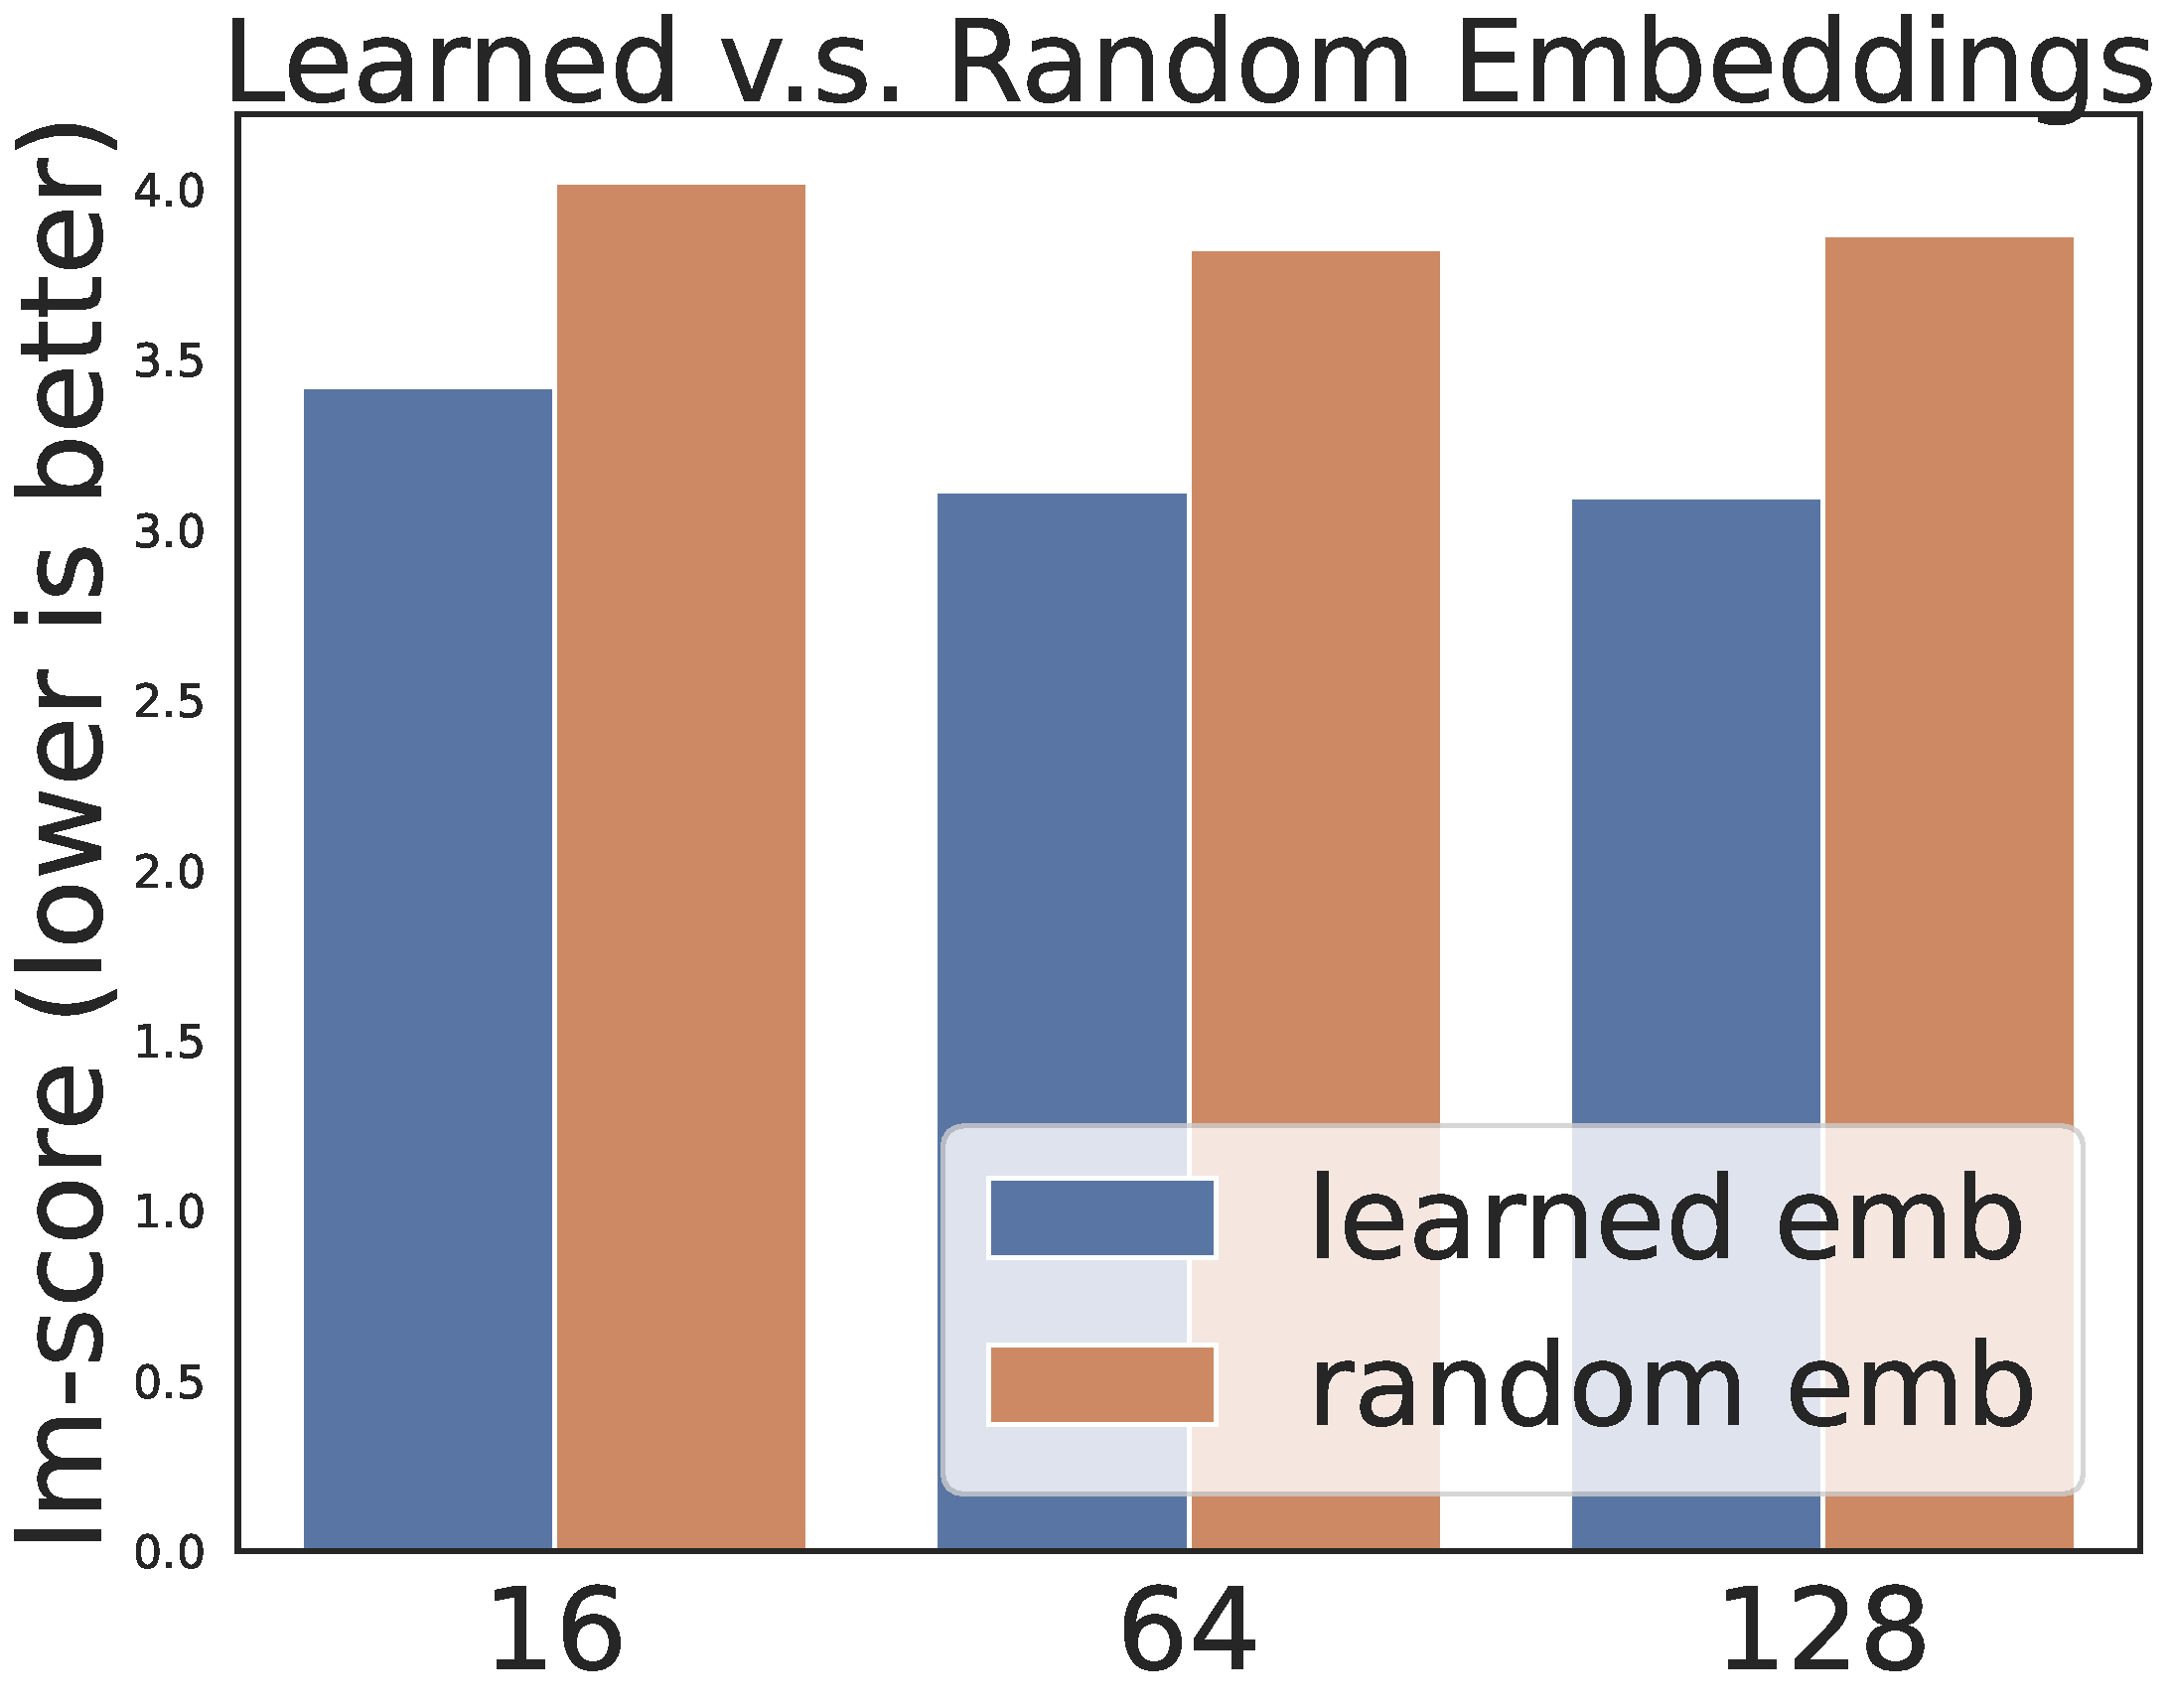
\includegraphics[width=0.25\textwidth]{fig/ablation_full1-2.pdf}
    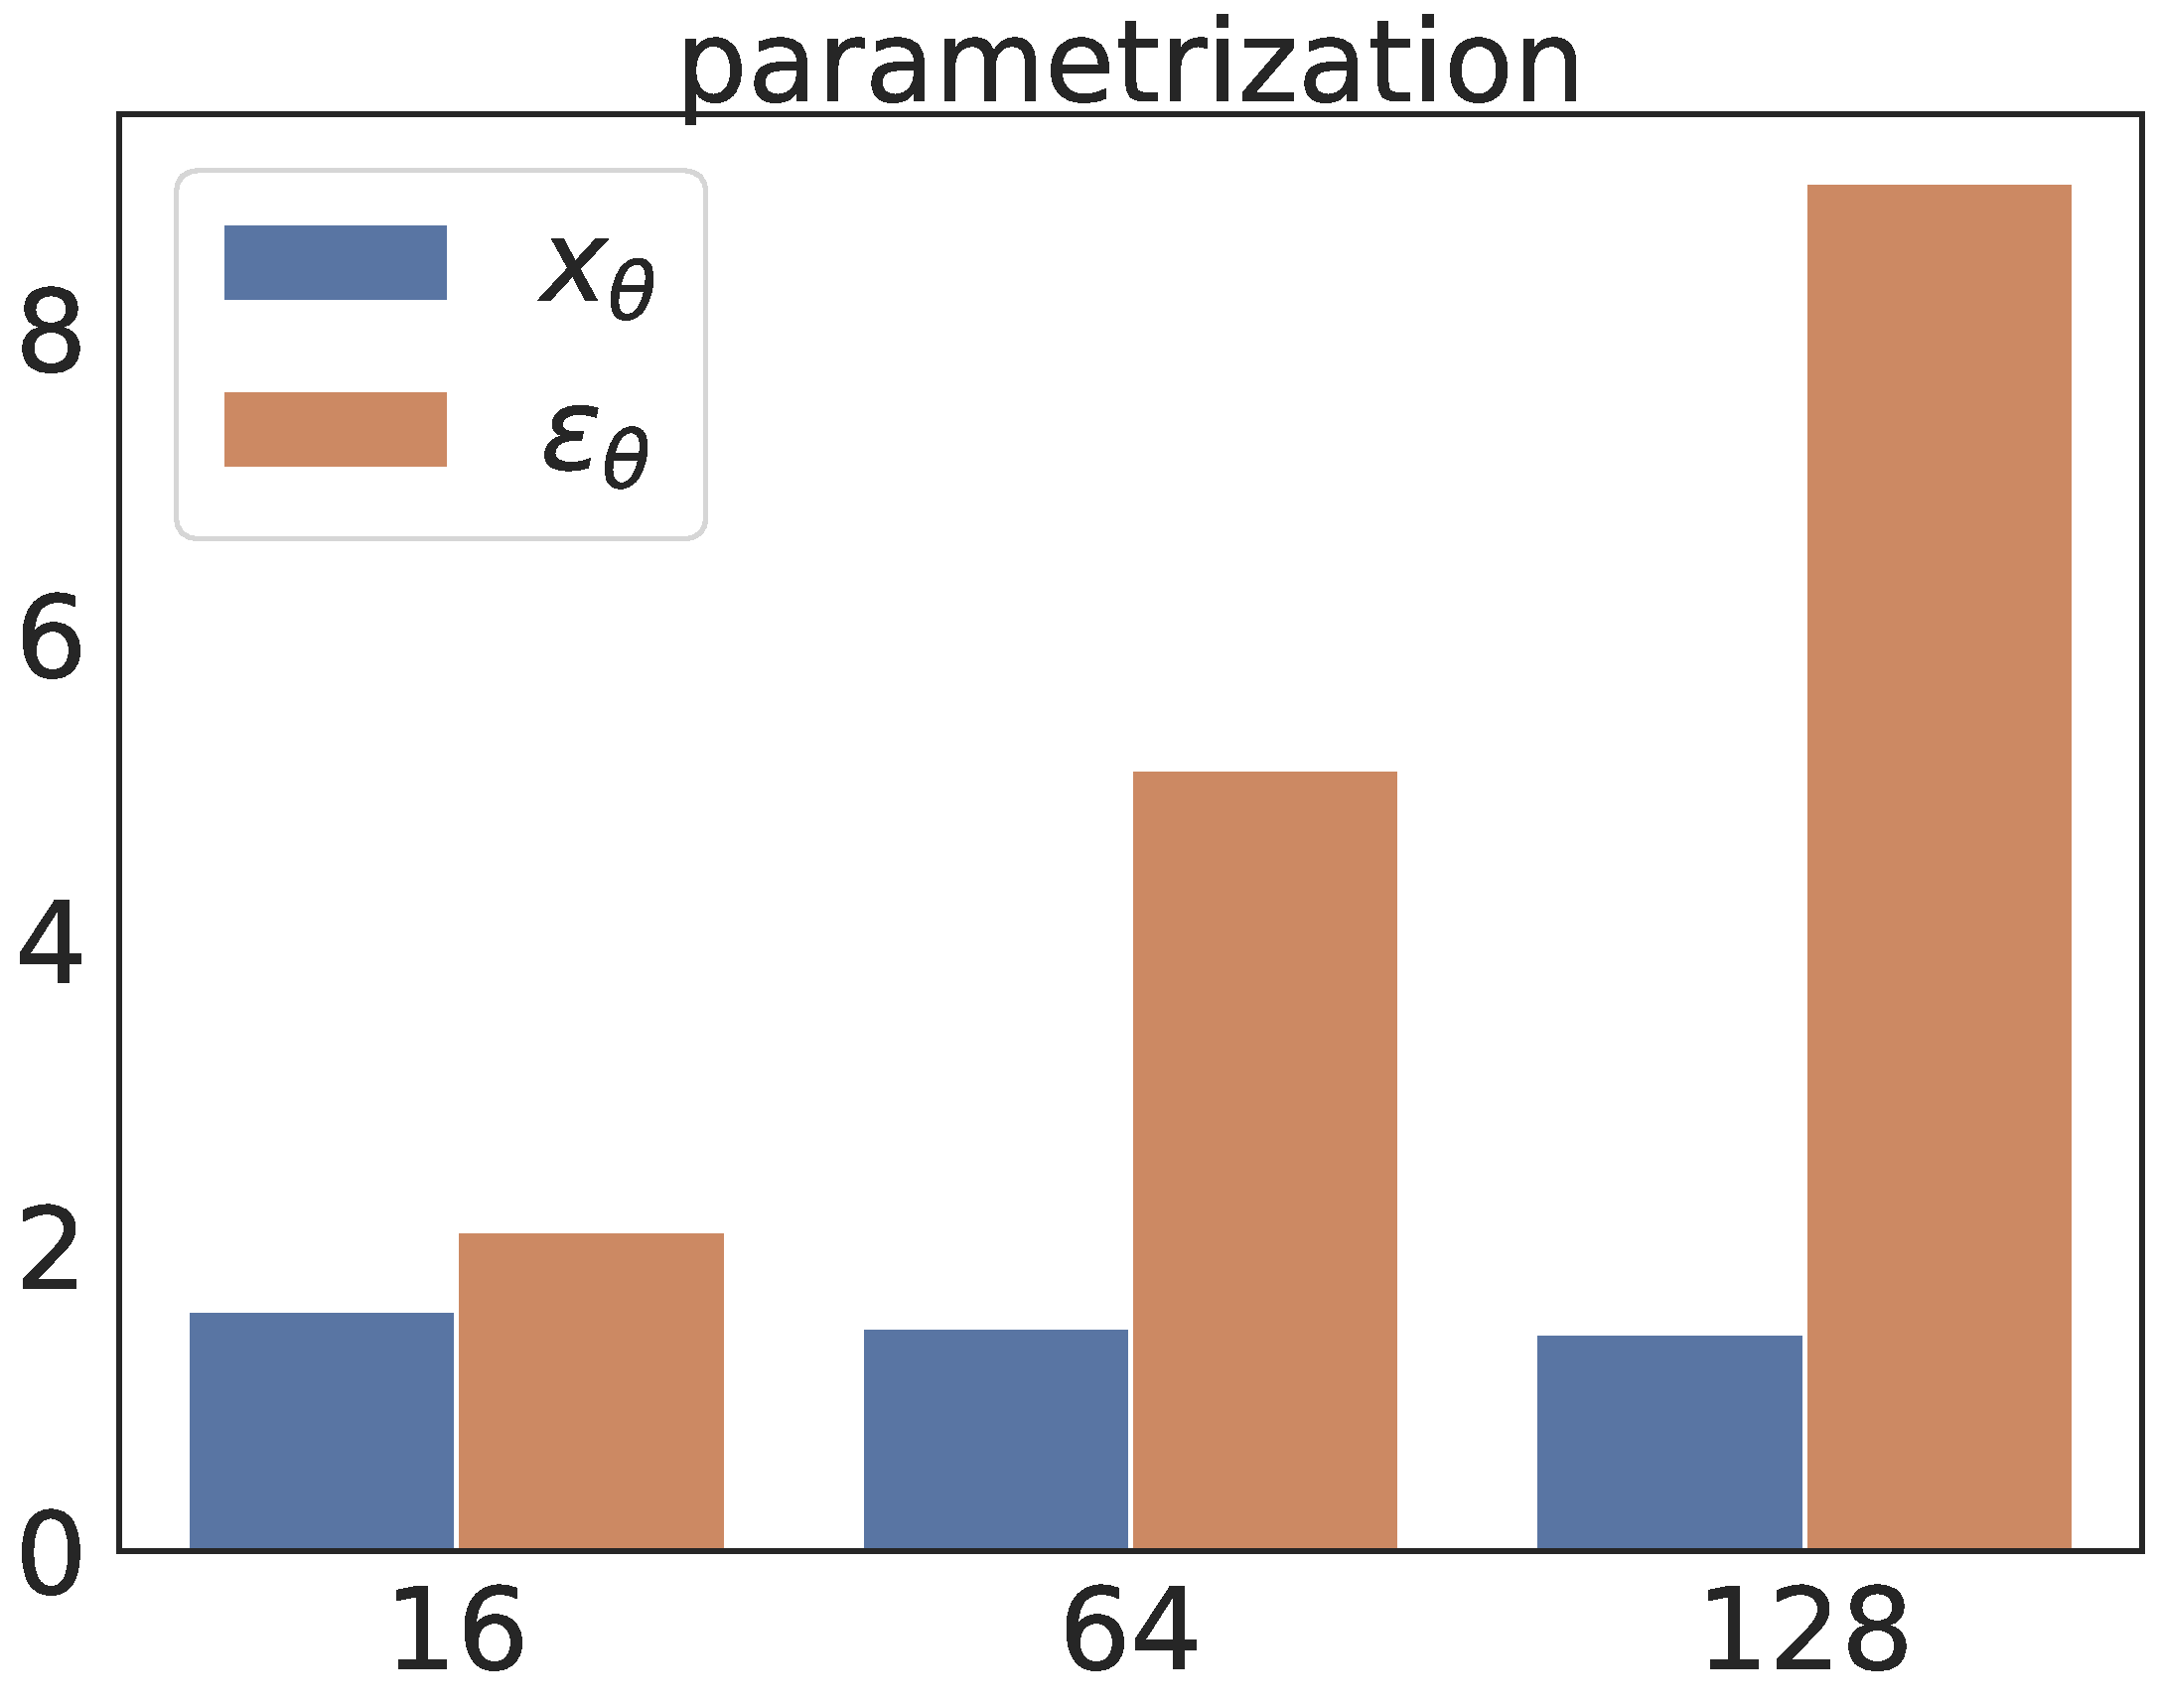
\includegraphics[width=0.25\textwidth]{fig/ablation_full2.pdf}
\caption{\label{fig:ablation}
제안한 설계 선택의 영향을 lm-score로 측정한다. 학습 임베딩과 재매개변수화 모두 표본 품질을 크게 향상시킴을 확인한다.
}
\end{wrapfigure}


\cref{sec:method}에서 제안한 설계 선택의 중요성을 두 가지 어블레이션으로 검증한다. \cref{ssec:control_gen_setup}처럼 500개 샘플의 lm-score로 Diffusion-LM의 표본 품질을 측정한다.

\textbf{학습 임베딩 vs.\ 랜덤 임베딩(\cref{ssec:embeddings}).}
더 어려운 언어모델링 과제인 ROCStories에서 학습 임베딩이 랜덤 임베딩을 능가한다. E2E 데이터셋에서도 같은 경향이지만 격차는 작다.


\textbf{목적함수 매개변수화(\cref{ssec:rounding}).}
디퓨전 모델이 $\cx{0}$를 직접 예측하도록 제안한다. 여기서는 이를 노이즈 항 $\epsilon$으로 매개변수화하는, 이미지 생성 분야의 표준 방식과 비교한다. \cref{fig:ablation}(오른쪽)은 $\cx{0}$ 매개변수화가 차원에 걸쳐 일관되게 좋은 성능을 내는 반면, $\epsilon$ 매개변수화는 작은 차원에서는 동작하지만 차원이 커지면 빠르게 붕괴함을 보여 준다.




\section{결론과 한계}
복잡하고 세밀한 제어 과제의 새로운 형태를 가능하게 하는, 연속 디퓨전 기반의 새로운 제어 가능 언어모델 Diffusion-LM을 제안하였다.
6개의 세밀 제어 과제에서 Diffusion-LM의 성공을 시연했다. 본 방법은 기존 방법의 제어 성공률을 거의 두 배로 끌어올리며, 추가 학습이 필요한 기준선 파인튜닝 방법과도 경쟁력이 있다.

Diffusion-LM이 가능하게 한 복잡한 제어는 매력적이며, Diffusion-LM이 현재의 이산 자기회귀 생성 패러다임에서 상당히 벗어났다는 점에서 우리는 고무되어 있다. 모든 새로운 기술이 그러하듯, 우리가 구성한 Diffusion-LM에도 단점이 있다. (1) perplexity가 더 높고, (2) 디코딩이 상당히 더 느리며, (3) 학습이 더 천천히 수렴한다. 후속 연구와 최적화를 통해 이러한 문제 다수가 해결될 수 있고, 본 접근이 대규모 제어 가능 생성의 유력한 방법이 될 것이라고 본다.



\begin{ack}
초기 논의와 피드백을 준 Yang Song, Jason Eisner, Tianyi Zhang, Rohan Taori, Xuechen Li, Niladri Chatterji, 그리고 p-lambda 그룹 구성원들께 감사드린다. PECASE 상의 지원에 깊이 감사드린다.
Xiang Lisa Li는 Stanford Graduate Fellowship의 지원을 받았다.
\end{ack}






\bibliography{anthology}



















\clearpage

 \appendix



\section{디퓨전 노이즈 스케줄}
\newcommand{\sqrtt}{\textit{sqrt}\xspace}
\newcommand{\cosine}{\textit{cosine}\xspace}
\newcommand{\linear}{\textit{linear}\xspace}

\label{app:noise}
\begin{wrapfigure}[11]{R}{0.25\textwidth}
\centering
\vspace{-10pt}
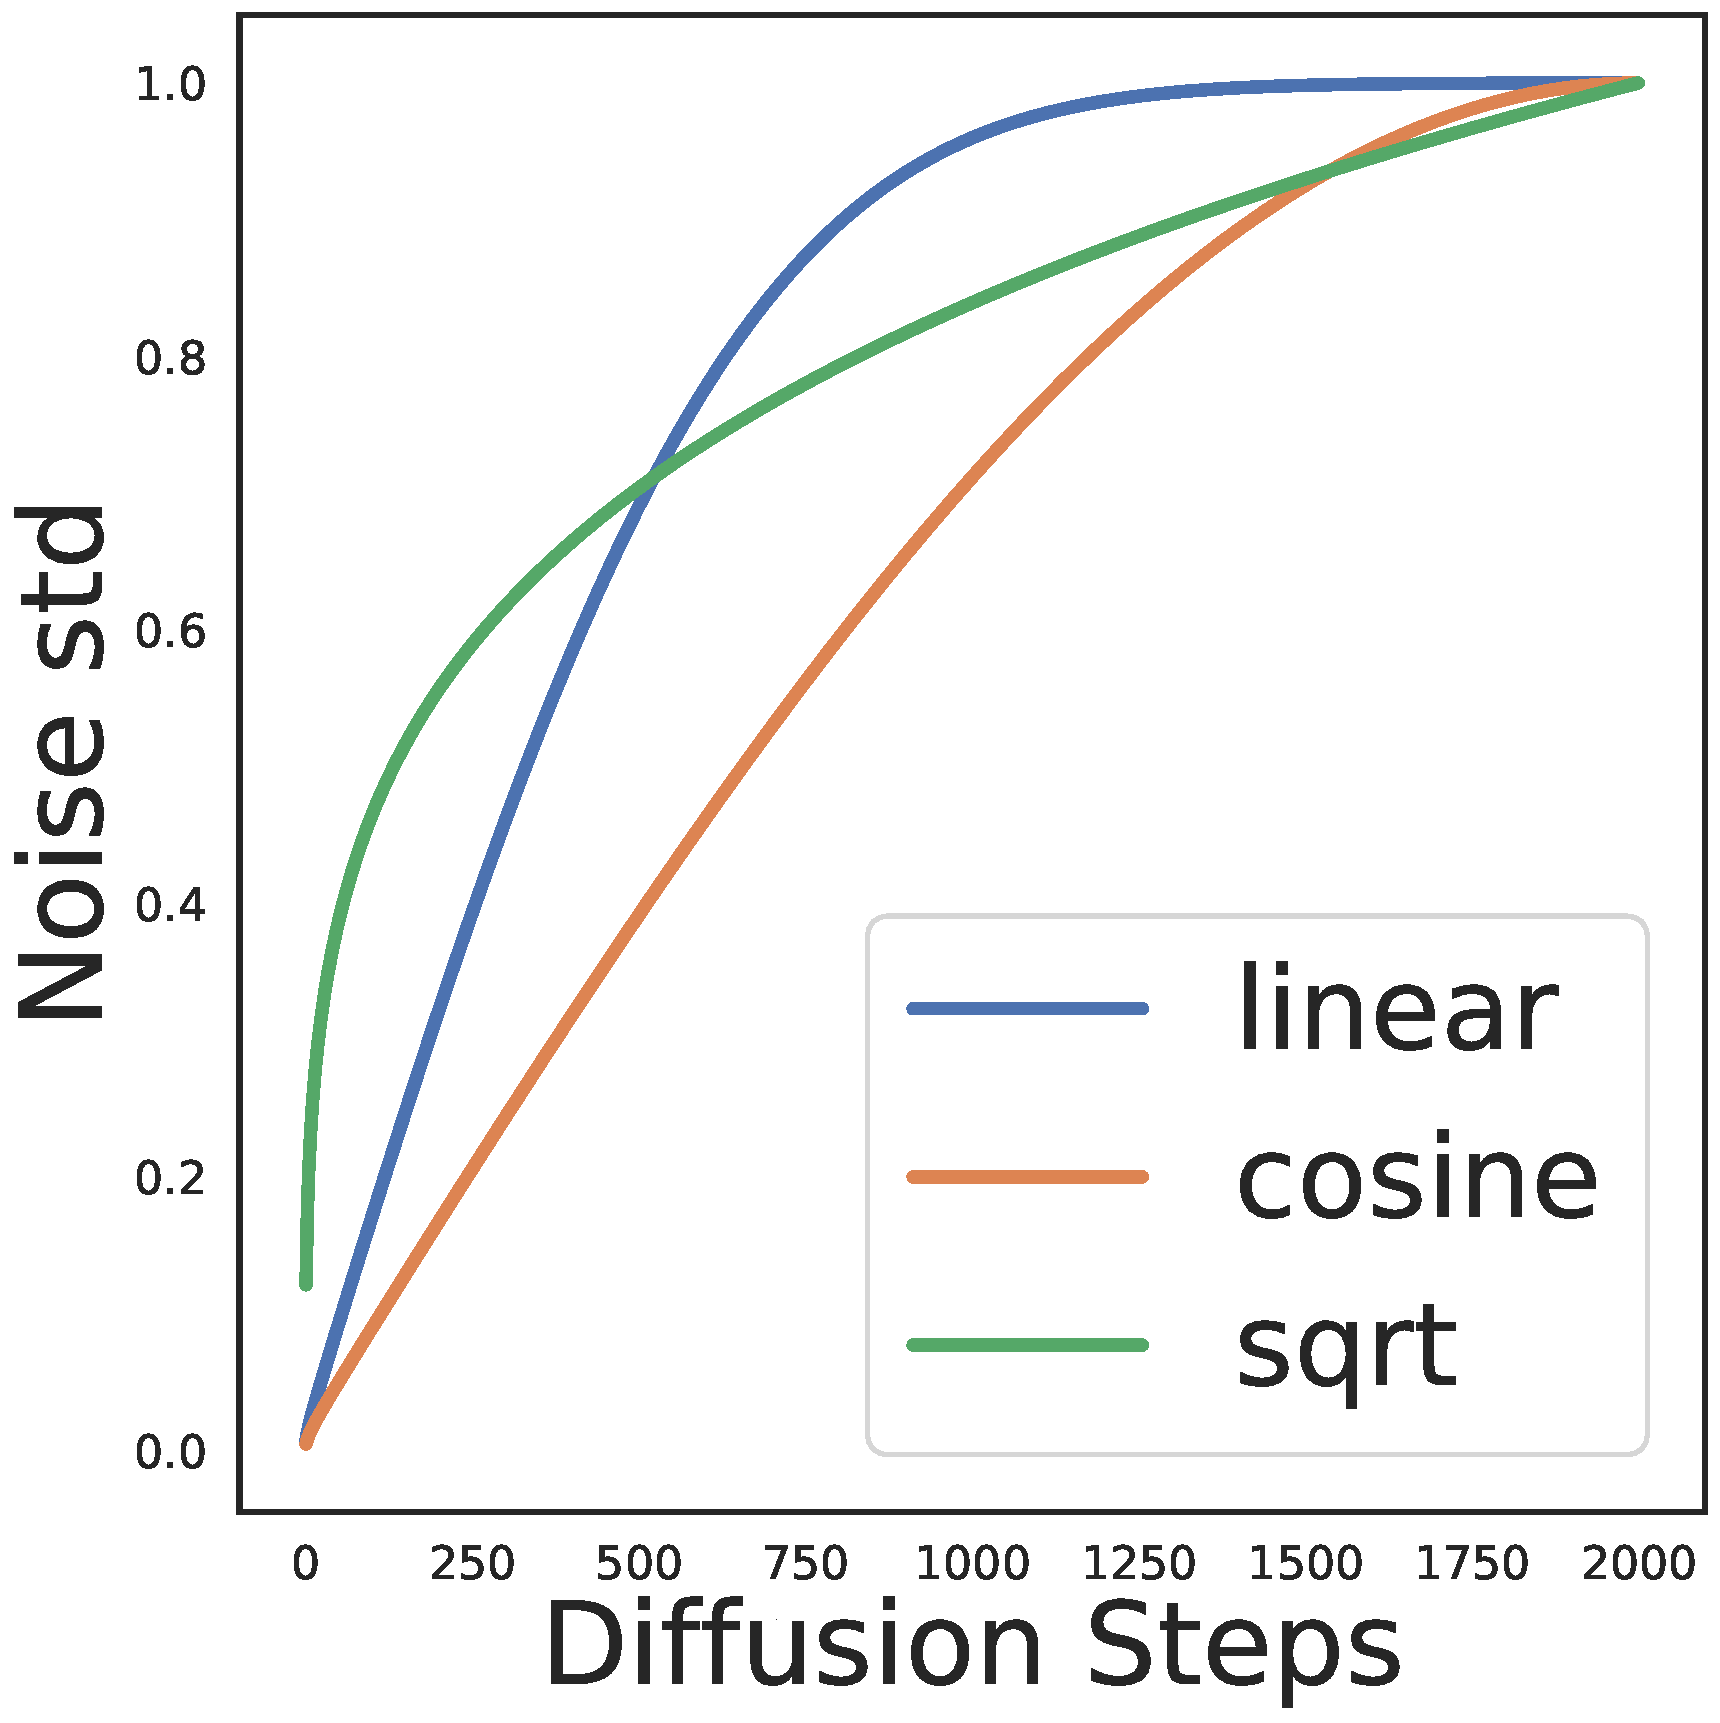
\includegraphics[width=0.9\linewidth]{fig/noise_schedule_v4.pdf}
\vspace{-3pt}
\caption{노이즈 스케줄 $\sqrt{1-\alphabar_t}$ 시각화. \label{fig:noise}}
\vspace{-10pt}
\end{wrapfigure}

디퓨전 모델은 모든 디퓨전 단계에 대해 파라미터를 공유하므로, 노이즈 스케줄($\alphabar_{1:T}$로 매개변수화)은 각 디노이징 문제에 얼마나 가중을 둘지 결정하는 중요한 하이퍼파라미터이다.
연속 디퓨전을 위한 표준 노이즈 스케줄은 텍스트 데이터에서 강건하지 않음을 확인했다. 우리는 텍스트의 이산성과 반올림 단계 때문에, 모델이 $t=0$ 근방의 노이즈에 둔감해진다고 가정한다. 구체적으로, 단어 임베딩에 작은 가우시안 노이즈를 더해도 임베딩 공간상 최근접 이웃이 거의 바뀌지 않으므로, $t=0$ 근방의 디노이징은 쉬운 과제가 된다.

이를 해소하기 위해 텍스트에 더 적합한 새로운 \sqrtt 노이즈 스케줄을 도입한다. \cref{fig:noise}에 나타냈고, $\alphabar_t = 1-\sqrt{t/T + s}$로 정의되며, $s$는 시작 노이즈 수준에 대응하는 작은 상수이다\footnote{우리는 $s=$1e-4, $T=2000$으로 설정하며, 이는 초기 표준편차를 $0.1$로 만든다.}. 표준 \linear, \cosine 스케줄에 비해 \sqrtt 스케줄은 더 높은 노이즈 수준에서 시작해 처음 50단계 동안 노이즈를 빠르게 증가시킨다. 그 후 \sqrtt는 노이즈 주입을 늦추어, 잘 풀기에 너무 어려울 수 있는 고노이즈 문제에 너무 많은 단계를 쓰지 않도록 한다.





\section{하이퍼파라미터}
\label{app:hyperparam}
\paragraph{Diffusion-LM 하이퍼파라미터.}
Diffusion-LM에 고유한 하이퍼파라미터에는 디퓨전 단계 수, Diffusion-LM의 아키텍처, 임베딩 차원, 노이즈 스케줄이 포함된다. 디퓨전 단계는 $2000$, 아키텍처는 BERT-base \cite{Devlin2019BERTPO}, 시퀀스 길이는 $64$로 설정한다.
임베딩 차원은 $d \in \{16, 64, 128, 256\}$ 중에서 선택하며, E2E 데이터셋에는 $d=16$, ROCStories에는 $d=128$을 선택한다.
노이즈 스케줄로는 \sqrtt 스케줄(\cref{app:noise})을 설계하였고, \cref{app:ablation}에서 보듯 다양한 매개변수화와 임베딩 차원에 더 강건하다. 다만 $\cx{0}$ 매개변수화(\cref{ssec:rounding})를 채택하고 나면 \sqrtt 스케줄의 이점은 두드러지지 않는다.

\paragraph{학습 하이퍼파라미터.}
AdamW 옵티마이저와 1e-4에서 시작하는 선형 감쇠 학습률, 드롭아웃 0.1, 배치 크기 64로 Diffusion-LM을 학습하며, 총 학습 반복 수는 E2E 데이터셋에서 20만, ROCStories에서 80만이다. 단일 GPU(NVIDIA RTX A5000, NVIDIA GeForce RTX 3090, NVIDIA A100)에서 학습한다. A100 한 장으로 20만 반복 학습에 약 5시간이 걸린다.

$\Lvlb^{\text{e2e}}$ 목적함수 하의 학습을 안정화하기 위해, 경사 클리핑을 1.0으로 설정하고 $\Lvlb$의 각 항을 재가중하는 중요도 샘플링 \cite{nichol2021improved}을 적용해야 한다. $\Lsimple^{\text{e2e}}$ 목적함수에서는 두 트릭 모두 필요 없다.

\paragraph{제어 가능 생성 하이퍼파라미터.} 제어 가능 생성을 위해 Diffusion-LM의 연속 잠재변수에 경사 갱신을 수행한다.
잠재변수 갱신에는 AdaGrad 옵티마이저 \cite{Duchi2010AdaptiveSM}를 사용하고, 학습률 $\text{lr} \in \{0.05, 0.1, 0.15, 0.2\}$와 트레이드오프 파라미터 $\lambda \in \{0.1, 0.01, 0.001, 0.0005\}$를 튜닝한다. 플러그앤플레이 제어 가능 생성 접근들은 서로 다른 하이퍼파라미터 튜닝으로 유창성과 제어를 절충한다. PPLM은 토큰당 경사 갱신 횟수 $k$를 사용하며 $k \in \{10, 30\}$을 튜닝한다. FUDGE는 트레이드오프 파라미터 $\lambda_{\text{FUDGE}}$를 사용하며 $\lambda_{\text{FUDGE}} \in \{16, 8, 4, 2 \}$를 튜닝한다. \cref{tab:hyper}에 각 제어 과제별로 선택된 하이퍼파라미터를 모두 나열한다. PPLM과 FUDGE의 추가 하이퍼파라미터는 원 논문의 지침을 따른다. PPLM의 학습률은 0.04, KL-scale은 0.01로 설정한다. FUDGE는 precondition top-K를 200, post top-K를 10으로 설정한다.

\newcommand{\tradeoff}{tradeoff}
\begin{table*}
\centering
\resizebox{0.9\columnwidth}{!}{
\begin{tabular}{lcc|cc|cc|cc|cc}
\toprule
          & \multicolumn{2}{c|}{Semantic} & \multicolumn{2}{c|}{Parts-of-speech} & \multicolumn{2}{c|}{Syntax Tree} & \multicolumn{2}{c|}{Syntax Spans} & \multicolumn{2}{c}{Length}  \\
& \tradeoff        & lr       & \tradeoff     & lr    & \tradeoff     & lr     & \tradeoff     & lr    &  \tradeoff     & lr    \\ \hline
PPLM      &  30  & 0.04  &  - & - & - & - & - & - & - &  - \\
FUDGE     & 8.0  & -  &20.0 & - & 20.0 & - & 20.0 & - & 2.0 & -  \\
Diffusion-LM & 0.01 & 0.1 & 0.0005 & 0.05 & 0.0005 & 0.2 &  0.1 & 0.15 & 0.01 & 0.1 \\
\bottomrule
\end{tabular}
}
\caption{\label{tab:hyper} 제어 가능 생성 방법의 하이퍼파라미터.}
\end{table*}

\section{디코딩 속도}
Diffusion-LM에서 표집하려면 2000 디퓨전 단계를 반복해야 하므로 $O(2000)$번의 $\xxtheta$ 모델 호출이 발생한다. 반면 자기회귀 LM의 표집은 시퀀스 길이 $n$에 대해 $O(n)$이다. 따라서 짧거나 중간 길이의 시퀀스 영역에서는 Diffusion-LM 디코딩이 자기회귀 LM 디코딩보다 느리다. 구체적으로 길이 64의 시퀀스 50개를 디코딩하는 데 약 1분이 걸린다.

디코딩을 가속하기 위해 생성 디퓨전 과정에서 단계를 건너뛰어 2000단계를 200단계로 다운샘플링하는 방법을 시도했다. 구체적으로 $T=200$으로 두고 노이즈 스케줄을 $\alphabar_{t} = \alphabar_{10t}$로 다운샘플링하는데, 이는 단위 전이를 $\cx{t} \rightarrow \cx{t+10}$ 전이로 두는 것과 같다. 새 노이즈 스케줄과 이산화로 Diffusion-LM을 디코딩한다. 이 단순한 접근은 E2E 같은 쉬운 언어모델링 과제에서는 표본 품질을 해치지 않지만, ROCStories 같은 어려운 과제에서는 품질이 떨어진다.

플러그앤플레이 제어 가능 생성 과제에서는 기존 접근들이 더 느리다.
PPLM은 토큰마다 30회의 경사 갱신을 수행하므로, 50 샘플 생성에 약 80분이 걸린다(배칭 없음).
FUDGE는 부분 시퀀스마다 가벼운 분류기를 호출해야 하므로 토큰당 200회의 분류기 호출, 결국 시퀀스 길이의 $100\times$ 호출이 필요하여 50 샘플 생성에 50초가 걸린다(배칭 있음). 분류기 호출은 배칭할 수 있지만, GPU 메모리 한계로 샘플 간 배칭이 제한될 수 있다.
우리 Diffusion-LM은 50 샘플 생성에 약 80초가 걸린다(배칭 있음). 본 방법은 디퓨전 단계 수를 200으로 다운샘플링하며, 디퓨전 단계당 분류기 호출이 3회이므로 총 600회의 모델 호출이 든다.

\section{분류기 유도 제어를 위한 분류기}
\textbf{의미 내용.} 텍스트를 조건으로 (필드, 값) 쌍을 예측하는 자기회귀 LM(GPT-2 small 아키텍처)을 학습한다. $\log p(\cc \mid \cx{t})$를 매개변수화하기 위해 ``value''의 토큰별 logprob을 계산한다.


\textbf{품사.} 분류기는 잠재변수에 조건화된 목표 POS 시퀀스의 확률을 추정하는 품사 태거로 매개변수화된다. 이 태거는 BERT-base 아키텍처를 사용한다. 입력은 연결된 단어 임베딩이고, 입력 단어마다 모든 POS 태그에 대한 소프트맥스 분포를 출력한다. $\log p(\cc \mid \cx{t})$는 시퀀스 안 각 단어의 POS log-prob의 합이다.

\textbf{구문 트리.} Transformer 기반 구성소(constituency) 파서 \cite{kitaev-klein-2018-constituency}를 학습한다. 본 파서는 각 스팬에 대해 국소 정규화된 예측을 수행하여 ``not a constituent'' 또는 구성소 라벨(예: 명사구(Noun Phrase))을 예측한다.
$\log p(\cc \mid \cx{t})$는 시퀀스 안 라벨링된 스팬과 비-구성소 스팬 각각의 log-prob 합이다.


\textbf{구문 스팬.} 구문 트리에 사용한 동일한 파서를 사용한다. $\log p(\cc \mid \cx{t})$는 목표 스팬이 목표 라벨로 주석되는 log-확률이다.

\section{종단간 목적함수 유도}
\label{app:derive}
연속 디퓨전 모델(\cref{ssec:diffusion_setup})에서 $\Lsimple$은 표준 목적함수 $\Lvlb$의 각 항을 재가중하여 유도된다.
$\Lvlb$의 처음 $T$개 항은 모두 두 가우시안 분포 사이의 KL 발산이며 닫힌 형식 해를 가진다. $t$번째 항을 예로 들면:
\begin{equation}
\mathop{\mathbb{E}}_{q(\cx{1:T} | \cx{0})} \left[ \log \frac{q(\cx{t-1} | \cx{0},\cx{t})} {\ptheta(\cx{t-1} | \cx{t}) }\right] = \mathop{\mathbb{E}}_{ q(\cx{1:T} | \cx{0})}  \left[ \frac{1}{2\sigma_t^2}  || \mu_\theta(\cx{t}, t) - \hat{\mu}(\cx{t}, \cx{0}) ||^2\right] + C, 
\label{app:eqn:simple}
\end{equation}
여기서 $C$는 상수, $\hat{\mu}$는 사후분포 $q(\cx{t-1} | \cx{0},\cx{t})$의 평균이며, $\mu_\theta$는 디퓨전 모델이 예측하는 $\ptheta(\cx{t-1} \mid \cx{t})$의 평균이다. 직관적으로, 이 단순화는 예측된 $\cx{t-1}$의 평균을 참 사후 평균에 맞춘다. 단순화는 상수 $C$와 스케일링 인자 $\frac{1}{2\sigma_t^2}$를 제거하여 $\Lsimple$의 한 항 $\mathop{\mathbb{E}}_{ q(\cx{1:T} | \cx{0})} \left[ || \mu_\theta(\cx{t}, t) - \hat{\mu}(\cx{t}, \cx{0}) ||^2\right]$를 얻는다.

이산 텍스트를 모델링하기 위해 연속 디퓨전을 적용하고자, Diffusion-LM(\cref{ssec:embeddings})을 설계하고, 디퓨전 모델과 임베딩 파라미터를 함께 학습하는 새로운 종단간 학습 목적함수(\cref{obj:e2e})를 제안한다. $\Lvlb^{\text{e2e}}$는 다음과 같이 풀어 쓸 수 있다.
\begin{align*}
    \mathcal{L}^\text{e2e}_{\text{vlb}} (\ww) &= \mathop{\mathbb{E}}_{q_\phi(\cx{0} | \ww)}\left[\mathcal{L}_{\text{vlb}} (\cx{0}) + \log \qphi(\cx{0} | \ww) - \log \ptheta(\ww | \cx{0})]\right] \\
    &= \mathop{\mathbb{E}}_{q_\phi(\cx{0:T} | \ww)}  \left[\underbrace{\log \frac{q(\cx{T} | \cx{0})}{\ptheta(\cx{T})}}_{L_T} + \sum_{t=2}^T \underbrace{\log \frac{q(\cx{t-1} | \cx{0},\cx{t})} {\ptheta(\cx{t-1} | \cx{t}) }}_{L_{t-1}} - \underbrace{\frac{\log \qphi(\cx{0} | \ww)}{\log \ptheta( \cx{0} | \cx{1})}}_{L_{0}}     - \underbrace{\log \ptheta(\ww | \cx{0})}_{L_\text{round}}\right]  \\
\end{align*}
$\Lvlb \rightarrow \Lsimple$로 변환하는 동일한 단순화를 적용해 $\mathcal{L}^\text{e2e}_{\text{vlb}} \rightarrow \Lsimpleee$로 변환한다.
\begin{align*}
    \mathop{\mathbb{E}}_{q_\phi(\cx{0:T} | \ww)} [L_T] & \rightarrow \mathbb{E}[||\mathop{\mathbb{E}}_{\cx{T}\sim q}[\cx{T}| \cx{0}] - 0 ||^2] = \mathbb{E}[||\hat{\mu}(\cx{T}; \cx{0})] ||^2] \\
    \mathop{\mathbb{E}}_{q_\phi(\cx{0:T} | \ww)} [L_{t-1}] & \rightarrow \mathbb{E}[|| \mathop{\mathbb{E}}_{\cx{t-1}\sim q}[\cx{t-1}| \cx{0}, \cx{t}] - \mathop{\mathbb{E}}_{\cx{t-1} \sim \ptheta}  [\cx{t-1} | \cx{t}] ||^2] =\mathbb{E}[ ||\hat{\mu}(\cx{t}, \cx{0})-\mu_\theta(\cx{t}, t) ||^2]\\
    \mathop{\mathbb{E}}_{q_\phi(\cx{0:T} | \ww)} [L_{0}] & \rightarrow \mathbb{E}[|| \mathop{\mathbb{E}}_{\cx{0}\sim\qphi} [\cx{0} \mid \ww] - \mathop{\mathbb{E}}_{\cx{0} \sim \ptheta} [\cx{0}  \mid \cx{1} ] ||^2] = \mathbb{E}[ ||\Emb(w)-\mu_\theta(\cx{1}, 1) ||^2]
\end{align*}

노이즈 스케줄이 $\alphabar_T = 0$을 만족하여 $\cx{T}$가 순수 가우시안 노이즈가 되면 첫 번째 항이 상수가 된다는 점에 유의하자.
반대로 $\cx{T}$가 순수 가우시안 노이즈가 되도록 노이즈 스케줄이 끝까지 가지 않는다면, 임베딩이 지나치게 큰 노름을 학습하는 것을 막기 위해 이 정규화 항을 포함해야 한다. 큰 노름의 임베딩은 퇴화 해(degenerate solution)이다. 다른 모든 디노이징 전이를 쉽게 예측 가능하게 만들지만, $p(\cx{T})$에서 정확하게 표집하는 것이 불가능해지기 때문이다.

이 항들을 결합하면 $\Lsimpleee$가 된다.
\begin{align*}
    \mathcal{L}^\text{e2e}_\text{simple} (\ww) & =  \mathop{\mathbb{E}}_{\qphi(\cx{0:T} | \ww)}  \left[||\hat{\mu}(\cx{T}; \cx{0})||^2 + \sum_{t=2}^T [||\hat{\mu}(\cx{t}, \cx{0})-\mu_\theta(\cx{t}, t) ||^2] \right] \\
& ~~~~~~~~~~~ + \mathop{\mathbb{E}}_{\qphi(\cx{0:1} | \ww)} \left[|| \Emb(\ww) - \mu_\theta(\cx{1}, 1) ||^2  - \log \ptheta(\ww | \cx{0})\right].
\end{align*}

직관적으로 우리는 입력 $(\cx{t}, t) \in (\mathbb{R}^{nd}, \mathbb{R})$를 받아 $\cx{t-1} \in \mathbb{R}^{nd}$의 분포를 예측하는 Transformer 모델을 학습한다. 이 Transformer 모델은 모든 디퓨전 단계 $t = 1\dots T$에 걸쳐 공유된다. $\Lsimpleee$의 유도에서 보였듯이, 가장 자연스러운 선택은 신경망이 $\cx{t-1} \mid \cx{t}$의 평균을 직접 예측하도록 매개변수화하는 것이며, 이를 $\mu_\theta$-매개변수화라 부른다.

스케일링 상수를 무시하면 $\mu_\theta$-매개변수화와 동치인 다른 매개변수화들도 있다. 예를 들어 \cref{ssec:rounding}에서처럼, Transformer 모델이 $\xxtheta(\cx{t}, t)$를 통해 $\cx{0}$를 직접 예측하도록 학습하고, 다루기 쉬운 가우시안 사후 $q(\cx{t-1} \mid \cx{0}, \cx{t})$로부터 $\cx{t-1}$의 평균을 계산할 수 있다. 이 평균은 예측된 $\cx{0}$와 관측된 $\cx{t}$에 조건화한 닫힌 형식 해 $\frac{\sqrt{\alphabar_{t-1}} \beta_t}{1-\alphabar_t}\cx{0} + \frac{\sqrt{\alpha_t} (1-\alphabar_{t-1})}{1-\alphabar_t} \cx{t}$를 갖는다.
\begin{align*}
& ||\hat{\mu}(\cx{t}, \cx{0})-\mu_\theta(\cx{t}, t) ||^2 \\
= &  ||(\frac{\sqrt{\alphabar_{t-1}} \beta_t}{1-\alphabar_t}\cx{0} + \frac{\sqrt{\alpha_t} (1-\alphabar_{t-1})}{1-\alphabar_t} \cx{t}) - (\frac{\sqrt{\alphabar_{t-1}} \beta_t}{1-\alphabar_t}\xxtheta(\cx{t}, t) + \frac{\sqrt{\alpha_t} (1-\alphabar_{t-1})}{1-\alphabar_t} \cx{t})||^2\\
= & ||\frac{\sqrt{\alphabar_{t-1}} \beta_t}{1-\alphabar_t}(\cx{0} - \xxtheta(\cx{t}, t))||^2\\
\propto &  ||\cx{0} - \xxtheta(\cx{t}, t)||^2
\end{align*}
두 매개변수화는 상수 스케일링만큼만 다르며, \cref{ssec:rounding}에서 논의한 대로 반올림 오차를 줄이기 위해 $\Lsimpleee$의 모든 항에 $\cx{0}$-매개변수화를 적용한다.
\begin{align*}
    \mathcal{L}^\text{e2e}_{\cx{0}\text{-simple}} (\ww) & =  \mathop{\mathbb{E}}_{\qphi(\cx{0:T} | \ww)}  \left[||\hat{\mu}(\cx{T}; \cx{0})||^2 + \sum_{t=2}^T [||\cx{0}-\xxtheta(\cx{t}, t) ||^2] \right] \\
& ~~~~~~~~~~~ + \mathop{\mathbb{E}}_{\qphi(\cx{0:1} | \ww)} \left[|| \Emb(\ww) - \xxtheta(\cx{1}, 1) ||^2  - \log \ptheta(\ww | \cx{0})\right].
\end{align*}

$\cx{0}$-매개변수화의 Diffusion-LM에서 샘플을 생성하려면, 각 디퓨전 단계에서 모델이 $\xxtheta (\cx{t}, t)$로 $\cx{0}$를 추정한 뒤 $q(\cx{t-1} \mid \xxtheta (\cx{t}, t), \cx{t})$에서 $\cx{t-1}$을 표집하고, 이를 다음 디퓨전 단계의 입력으로 넣는다.






\section{로그가능도 모델과 결과}
\label{app:simplex}

Diffusion-LM의 로그가능도 성능을 살펴보기 위해 \cref{sec:method}의 학습 절차에서 몇 가지를 변경한다.
결과적으로 본 절에서 설명하는 로그가능도 개선은 우리의 실험에서 더 나은 생성 품질로 이어지지 않았으므로, 논문의 나머지 부분에서는 원래의 방법에 집중한다.
가능도 모델은 다음과 같이 학습한다.
\begin{itemize}
    \item 저차원 토큰 임베딩 시퀀스에서 디퓨전 모델을 학습하는 대신, 원-핫(one-hot) 토큰 벡터 시퀀스에서 직접 모델을 학습한다.
    \item \citet{kingma2021variational}의 설정을 따라 연속 시간 디퓨전 모델을 로그가능도 한계에 대해 학습하고, 손실 분산을 최소화하도록 노이즈 스케줄을 모델의 나머지와 함께 학습한다.
    \item 모델이 원-핫 벡터 시퀀스를 예측하므로 출력에 소프트맥스 비선형성을 사용하며, 손실의 모든 제곱오차 항을 교차 엔트로피 항으로 대체한다. 이 대리 손실 선택이 최적화에 더 유리했지만, 평가는 원래의 제곱오차 손실로 한다.
    \item 모델은 모든 Transformer 레이어 이전에 다음 변환을 입력에 적용한다: $x := \mathrm{softmax}(\alpha(t) x + \beta(t))$. 여기서 $\alpha(t) \in \mathbb{R}$, $\beta(t) \in \mathbb{R}^v$는 디퓨전 시간 단계 $t$의 함수이며 MLP로 매개변수화된다($v$는 어휘 크기).
    \item 추론 시에는 \cref{ssec:rounding}의 반올림 절차를 생략한다.
\end{itemize}
정확한 모델 아키텍처와 학습 하이퍼파라미터는 공개 코드를 참고하라.

이 디퓨전 모델들과 기준선 자기회귀 Transformer를 E2E와 ROCStories에서 학습하고, \cref{tab:ppl}에 로그가능도를 보고한다.
대략 1억 파라미터의 ``small'' 모델과 약 3억 파라미터의 ``medium'' 모델 두 크기의 Transformer를 학습한다.
E2E와 ROCStories는 데이터셋이 충분히 작아 모든 모델이 학습 초반에 최소 테스트 손실에 도달한다(이후 과적합).
대규모 데이터셋 환경에서의 모델 성능을 추가로 비교하기 위해 ``ROCStories (+GPT-J)'' 실험도 제시한다. 원본 ROCStories 데이터로 GPT-J \citep{gpt-j}를 파인튜닝하여 800만 건의 합성 ROCStories 학습 데이터를 생성하고, 합성 데이터셋에서 모델을 사전학습한 뒤 원본 ROCStories 데이터로 파인튜닝·평가한다.

\begin{table*}
    \centering
\begin{tabular}{lcc|cc|cc|cc|cc}
\toprule
    Dataset                & Small AR    & Small Diffusion     & Medium Diffusion\\
    E2E                    & 1.77    & 2.28 & -\\
    ROCStories             & 3.05    & 3.88 & -\\
    ROCStories (+GPT-J)    & 2.41    & 3.59 & 3.10\\

\bottomrule
\end{tabular}
\caption{\label{tab:ppl} 로그가능도 결과(토큰당 nats)}
\end{table*}

\section{정성적 예시}
\label{app:qualitative}

비조건 생성과 5개 제어 과제에 대한 Diffusion-LM의 무작위 샘플 출력을 보인다. \cref{app:qualitative-unc}은 비조건 생성 결과이다.
\cref{app:qualitative-span}, \cref{app:qualitative-pos}, \cref{app:qualitative-content}, \cref{app:qualitative-syntax}는 각각 스팬 제어, POS 제어, 의미 내용 제어, 구문 트리 제어의 정성적 샘플을 보인다.
\cref{app:qualitative-length}은 길이 제어의 결과이다. \emph{샘플 텍스트는 모델이 생성한 영어 출력 그대로 둔다.}


\section{추가 어블레이션 연구}
\label{app:ablation}
\cref{sec:ablation}의 2개 어블레이션 외에, \cref{app:tab:ablation}에 아키텍처 선택과 노이즈 스케줄에 관한 추가 어블레이션 결과를 제공한다.

\textbf{학습 임베딩 vs.\ 랜덤 임베딩(\cref{ssec:embeddings}).}
\cref{app:tab:ablation}의 첫 행에서 보듯, 학습 임베딩이 ROCStories와 E2E 데이터셋 모두에서 랜덤 임베딩을 각각 약간 능가한다.


\textbf{노이즈 스케줄(\cref{app:noise}).}
\sqrtt 스케줄을 이미지 모델링용으로 제안된 \cosine \cite{nichol2021improved}, \linear \cite{ho2020denoising} 스케줄과 비교한다. \cref{app:tab:ablation}의 가운데 행은 \sqrtt 스케줄이 모든 차원과 매개변수화 선택에 걸쳐 일관되게 좋고 안정적인 성능을 달성함을 보여 준다. $\cx{0}$ 매개변수화에서는 \sqrtt 스케줄의 중요성이 덜하지만, $\epsilon$ 같은 대안 매개변수화에서는 훨씬 더 강건한 노이즈 스케줄을 제공한다.

\paragraph{Transformer vs.\ U-Net.}
\citet{ho2020denoising}의 U-Net 아키텍처는 2D 합성곱 레이어를 사용하며, 우리는 텍스트 데이터에 적합한 1D 합성곱으로 바꾸는 것 외에는 모든 모델 아키텍처를 모방한다.
\cref{app:tab:ablation}(마지막 행)은 Transformer 아키텍처가 U-Net을 능가함을 보인다.

\begin{figure}

 \vspace{-10pt}
    \centering
    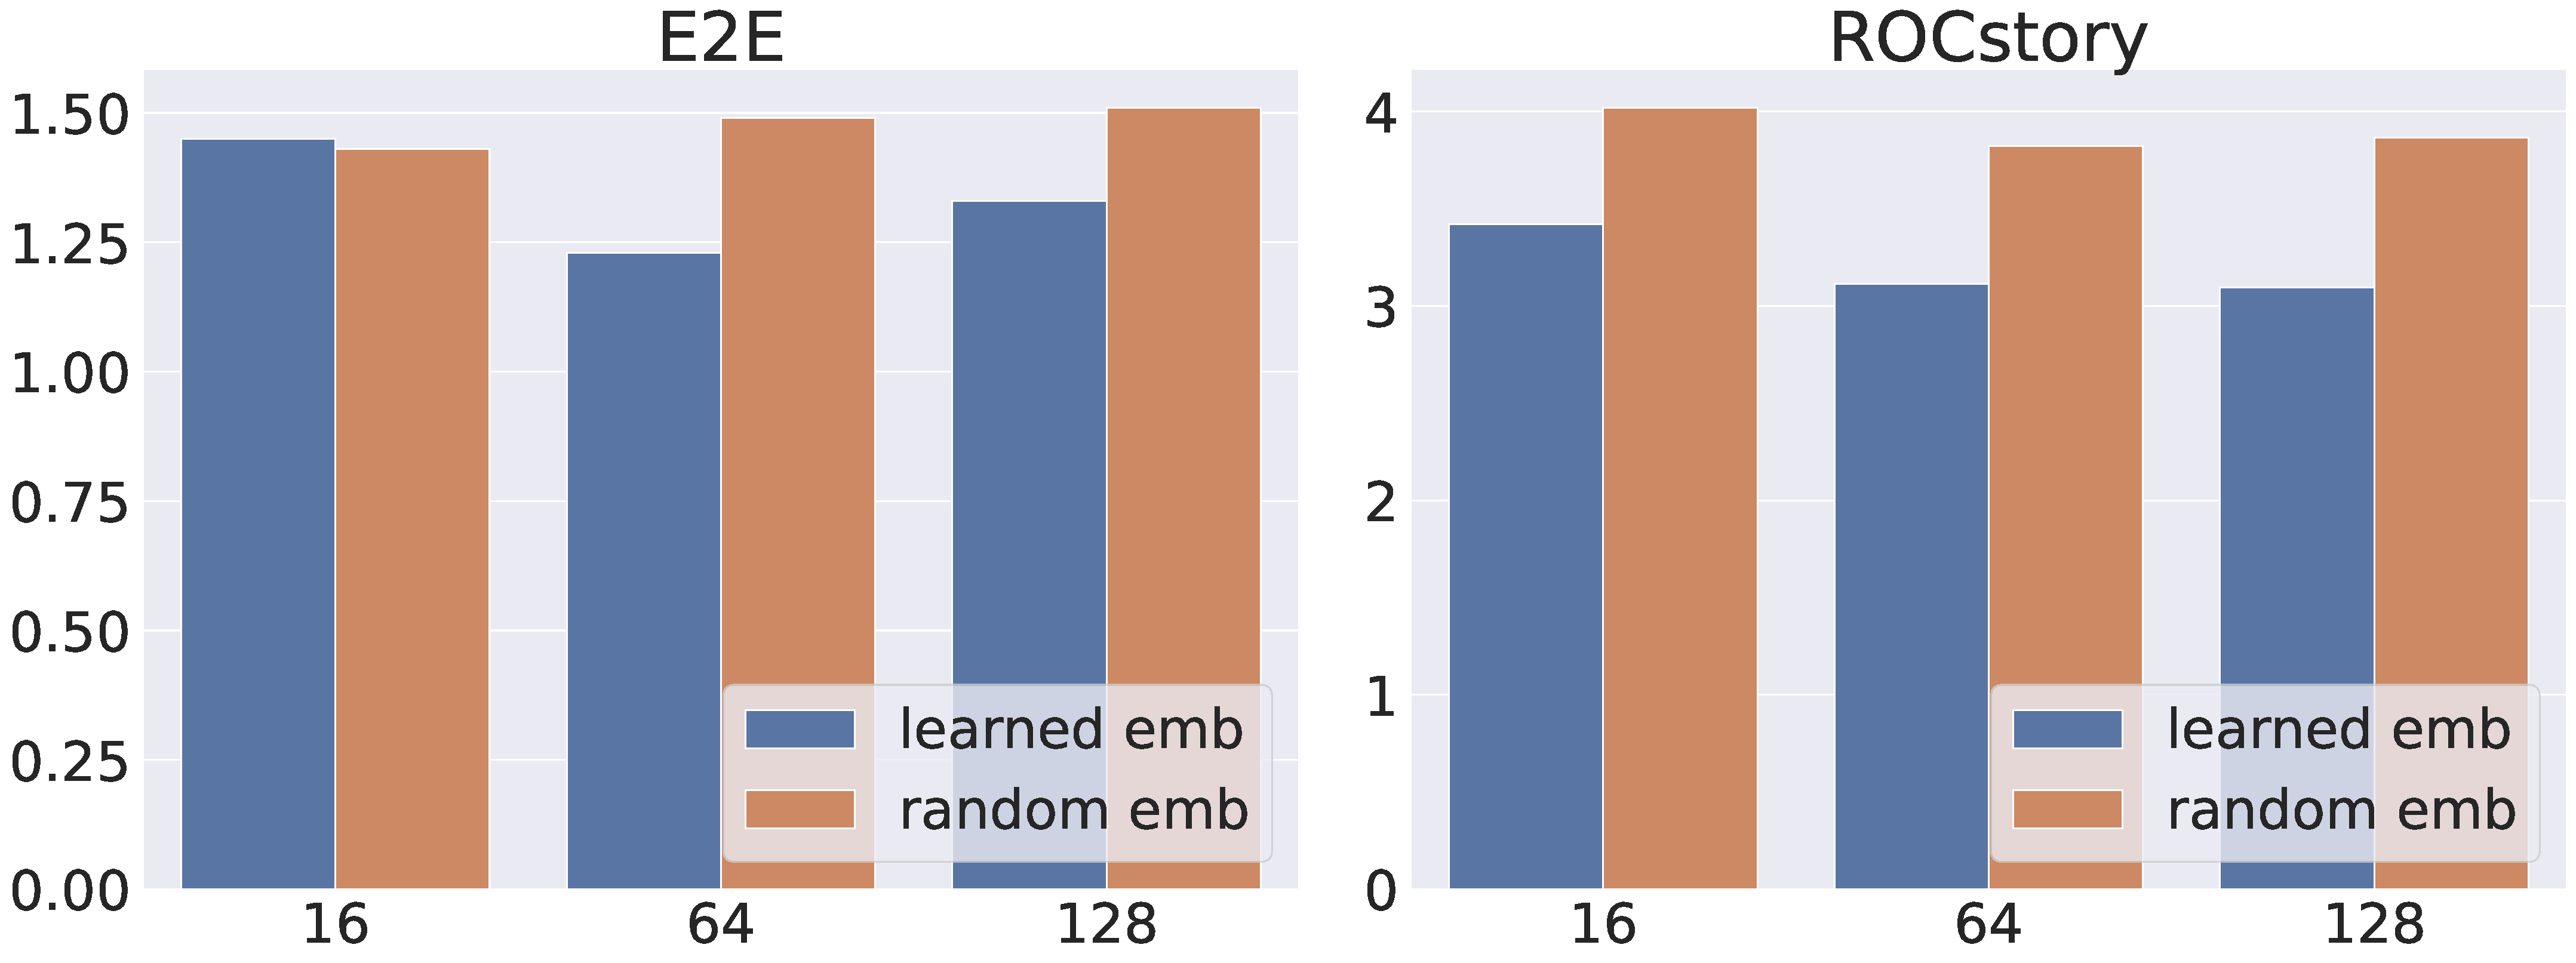
\includegraphics[width=0.8\textwidth]{fig/ablation_emb_e2e_appendix.pdf}
    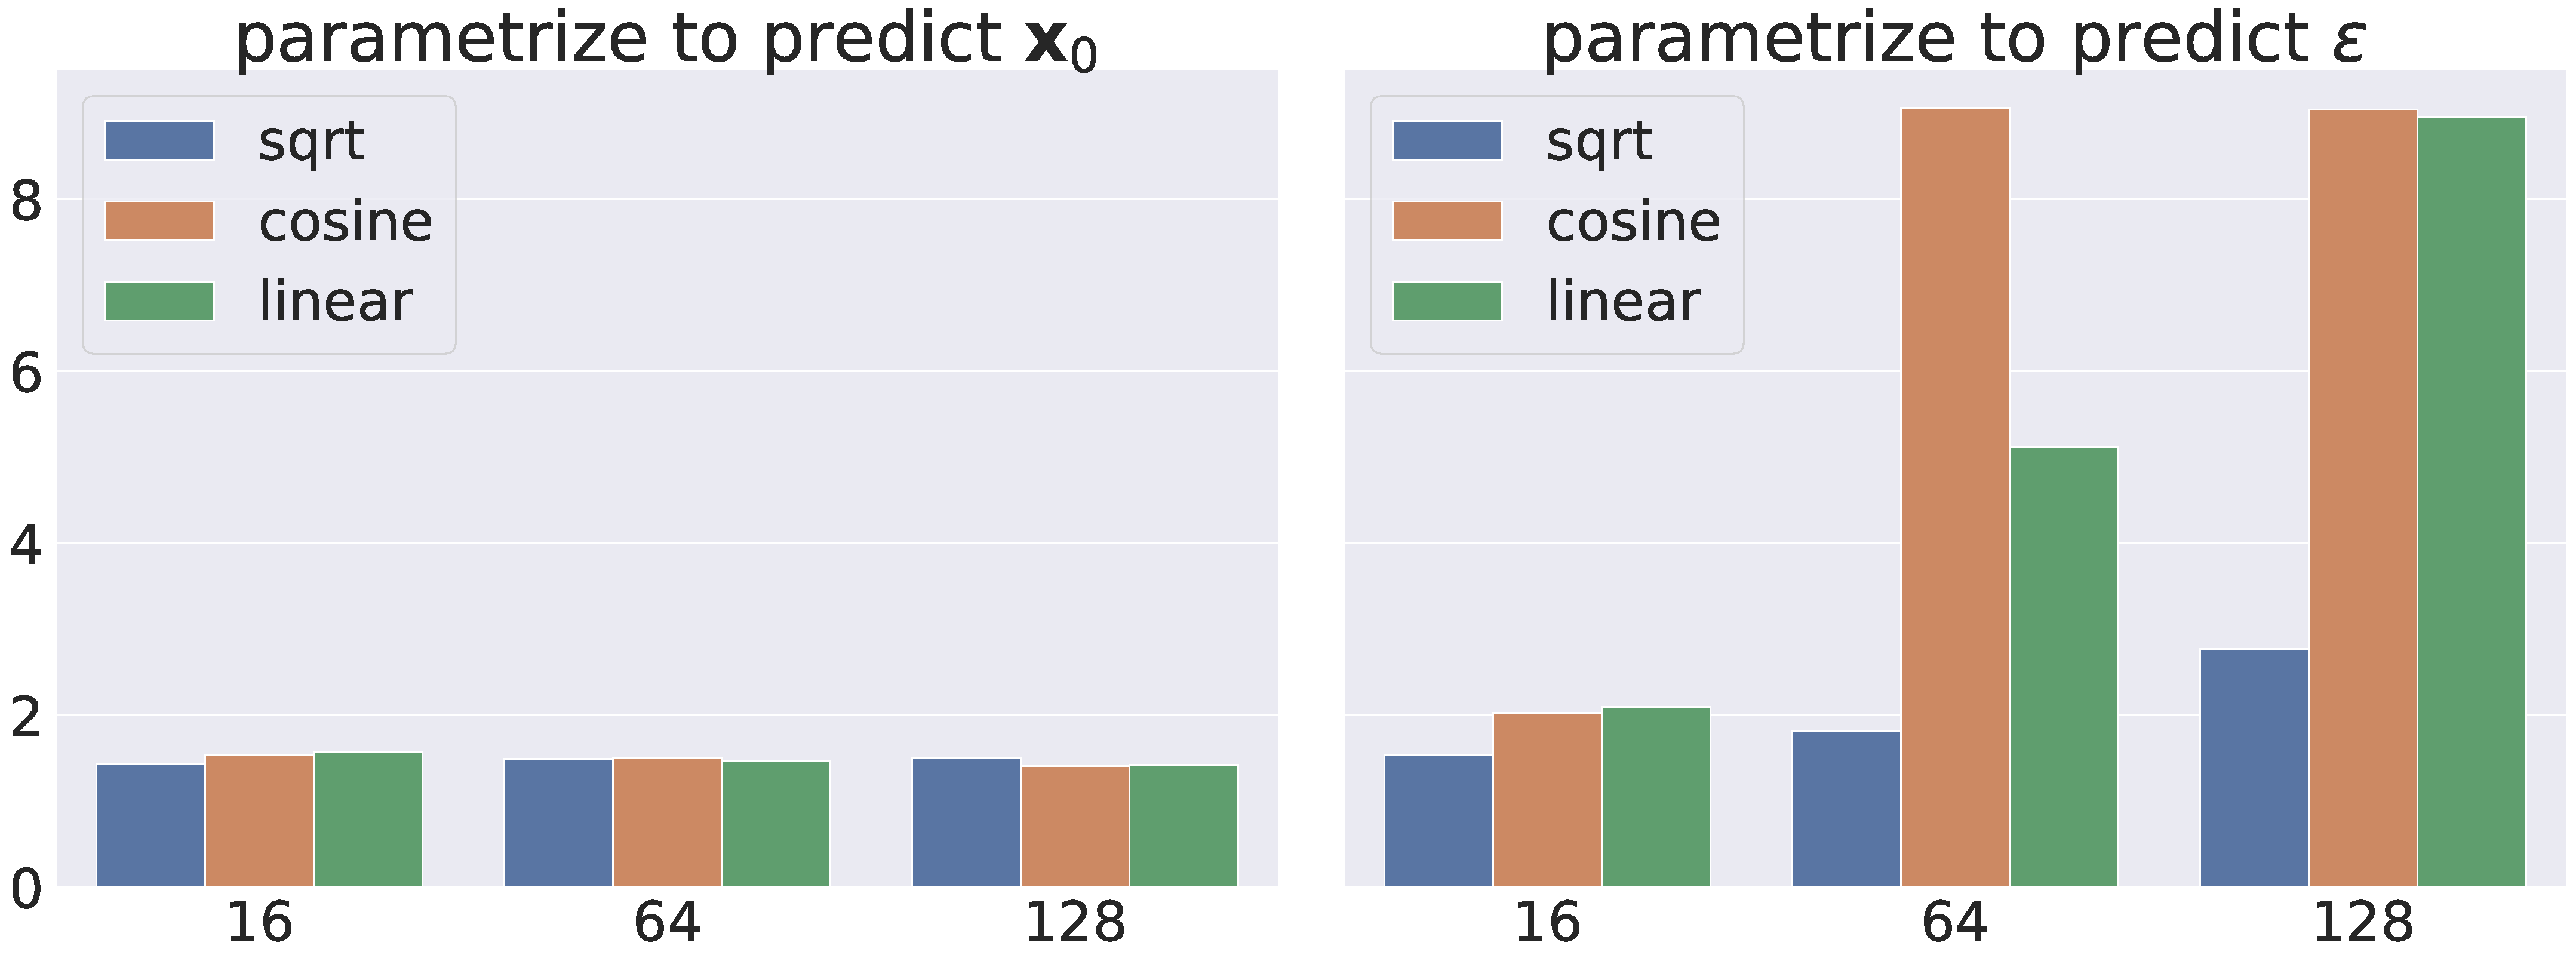
\includegraphics[width=0.8\textwidth]{fig/ablation_parametrization_appendix.pdf}
    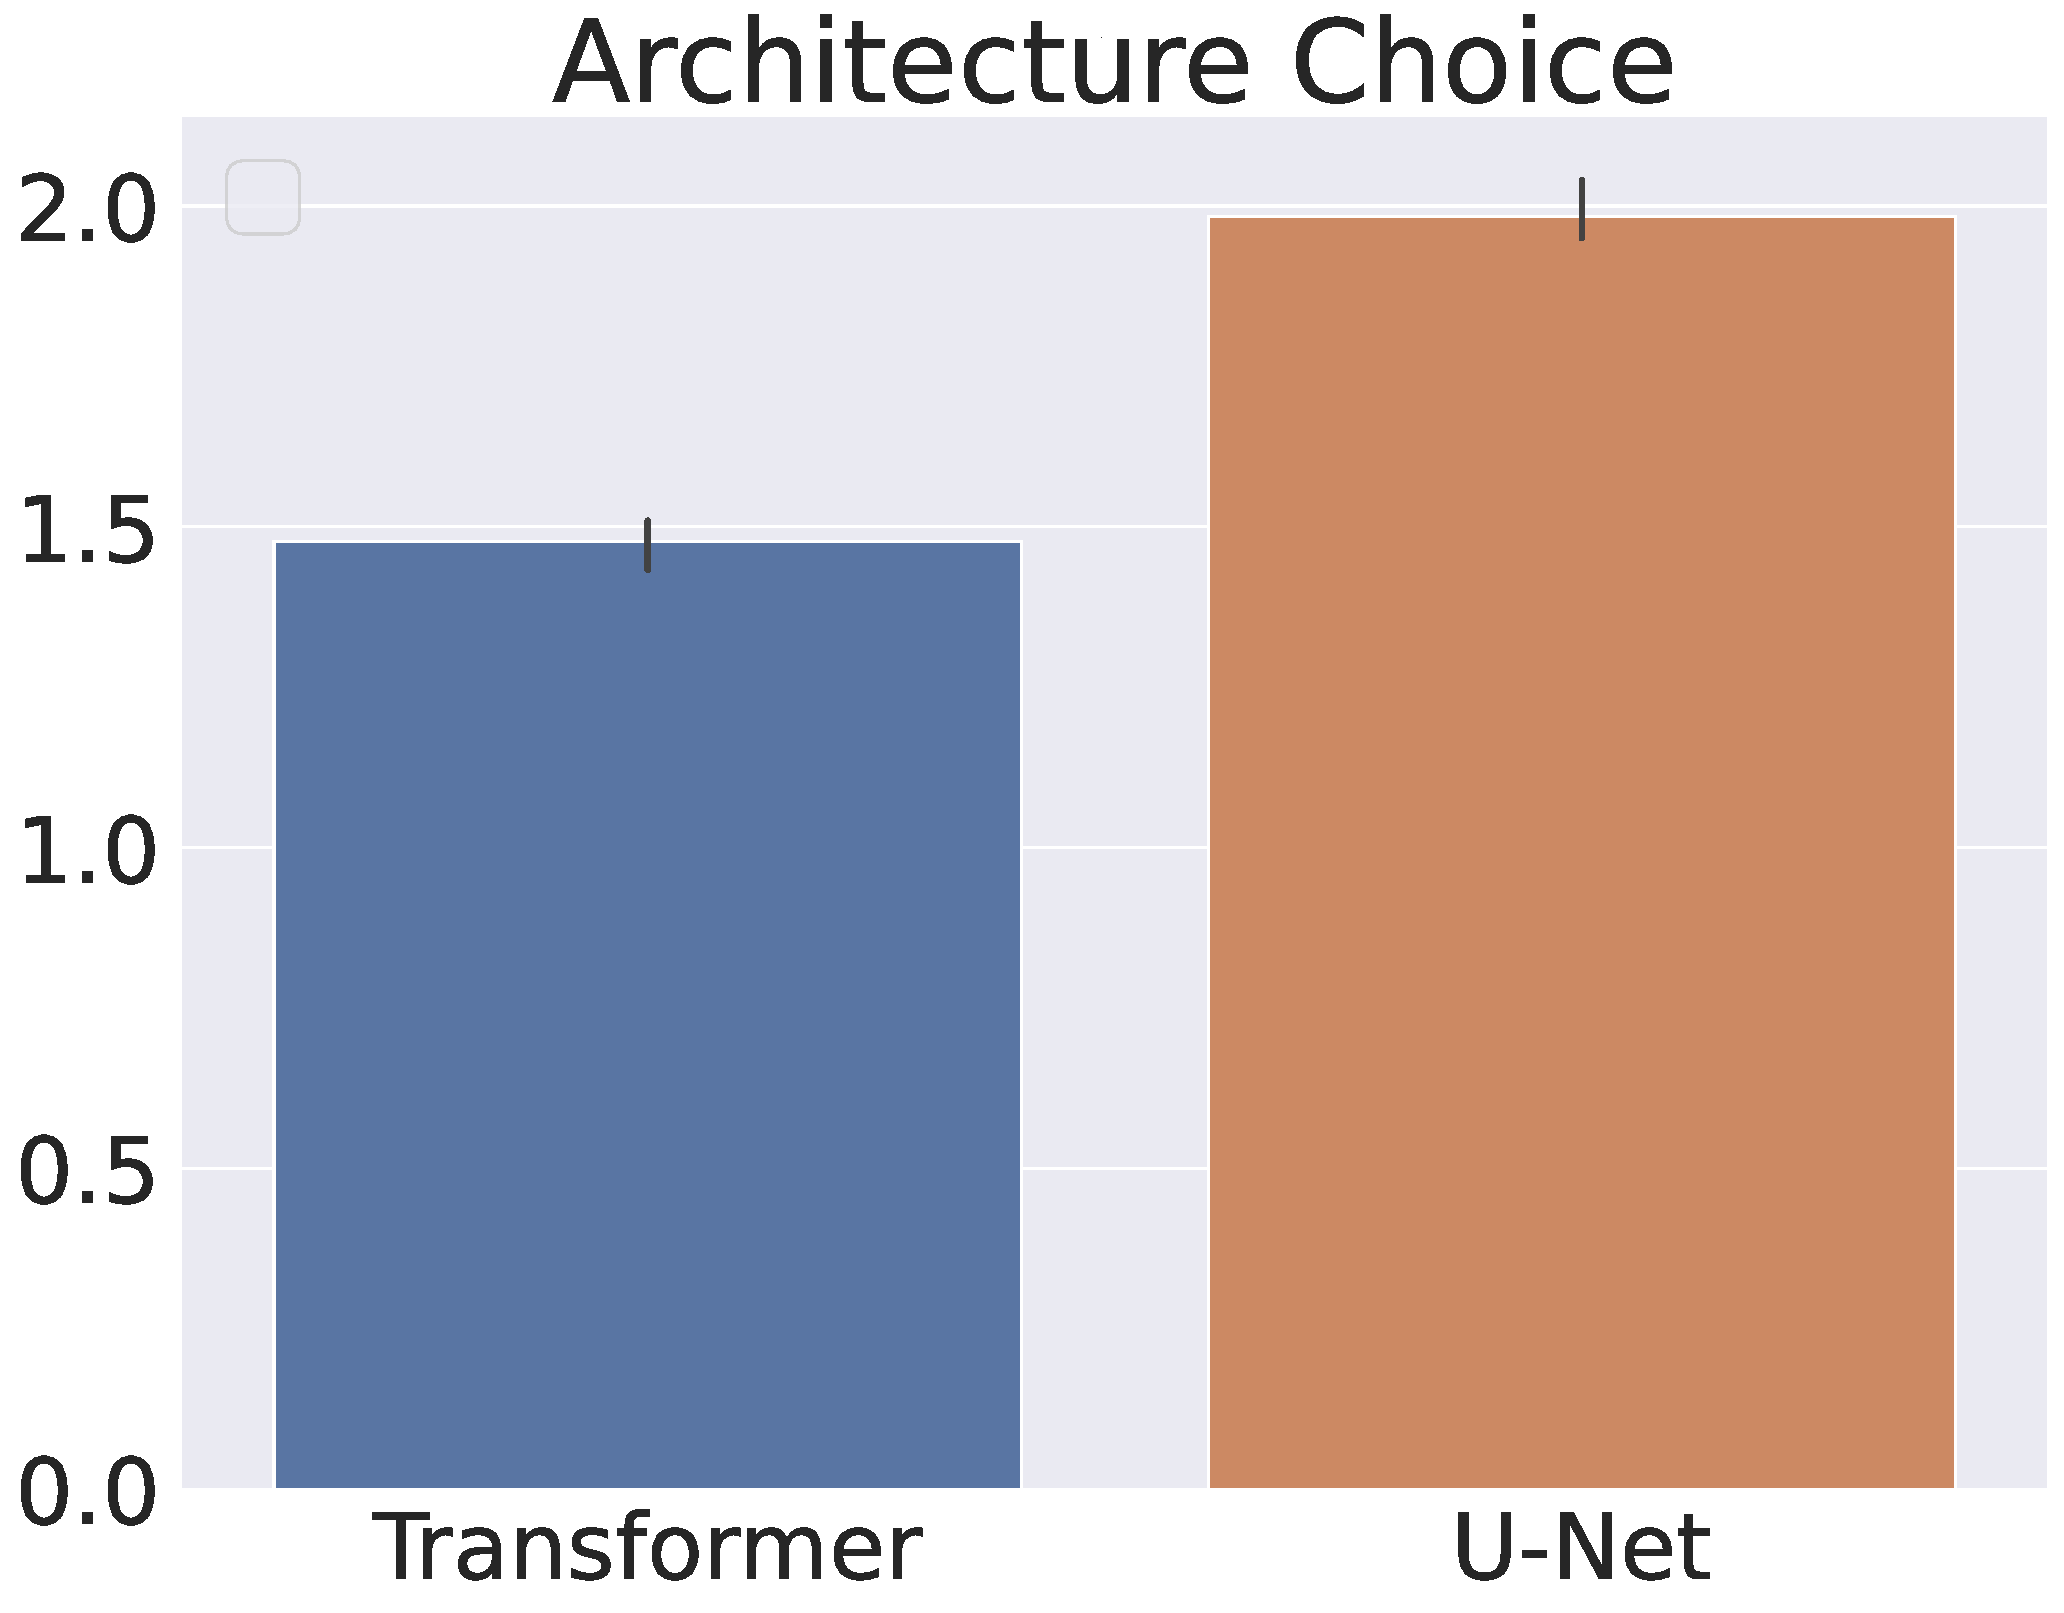
\includegraphics[width=0.4\textwidth]{fig/ablation_architecture_appendix.pdf}
\caption{\label{app:tab:ablation} 추가 어블레이션 결과. 첫 행은 학습 가능한 임베딩의 Diffusion-LM이 두 데이터셋 모두에서 랜덤 임베딩을 능가함을 보인다(\cref{ssec:embeddings}). 둘째 행은 \sqrtt 스케줄이 모든 차원·매개변수화 선택에서 일관되게 좋고 안정적인 성능을 달성함을 보여 준다. 마지막 행은 언어모델링에서 Transformer 아키텍처가 U-Net 아키텍처를 능가함을 보인다.
}
\end{figure}


\section{사회적 영향}
한편으로, 언어모델의 강한 제어 가능성은 독성을 완화하여 모델 배포를 더 안정적으로 만들 수 있다. 또한 모델이 더 진실하도록 제어함으로써 언어모델이 생성하는 부정확한 정보를 줄일 수도 있다.
다른 한편으로, 세밀한 제어 가능성에서 유래하는 보다 강력한 표적형 허위정보(예: 서사 쐐기 박기)도 상상할 수 있다.

이 점에서, 유창성에 영향을 주지 않으면서 생성 출력에 워터마크를 새길 수 있는 생성 방법을 고려할 가치가 있다. 이러한 워터마킹 또한, 식별 가능성과 유창성을 제약 조건으로 두는 제어 가능 생성 문제로 볼 수 있다.

\FloatBarrier

\begin{table*}
    \centering
    \resizebox{1\linewidth}{!}{
    \begin{tabular}{lp{13cm}}
\toprule
\parbox[t]{2mm}{\multirow{5}{*}{\rotatebox[origin=c]{90}{ROCStories+Aug}}} & Matt was at the store . He was looking at a new toothbrush . He found the perfect one . When he got home , he bought it . It was bright and he loved it . \\\\
& I and my friend were hungry . We were looking for some to eat . We went to the grocery store . We bought some snacks . We decided to pick up some snacks . \\\\
& I was at the store . I had no money to buy milk . I decided to use the restroom . I went to the register . I was late to work . \\\\
& The man wanted to lose weight . He did n't know how to do weight . He decided to start walking . He ate healthy and ate less . He lost ten pounds in three months . \\\\
& I went to the aquarium . I wanted to feed something . I ordered a fish . When it arrived I had to find something . I was disappointed .\\
\toprule
\toprule
\parbox[t]{2mm}{\multirow{5}{*}{\rotatebox[origin=c]{90}{ROCStories}}} & Tom was planning a trip to California . He had fun in the new apartment . He was driving , until it began to rain . Unfortunately , he was soaked . Tom stayed in the rain at the beach . \\\\
& Carrie wanted a new dress . She did not have enough money . She went to the bank to get one , but saw the missed . Finally , she decided to call her mom . She could not wait to see her new dress . \\\\
& Tina went to her first football game . She was excited about it . When she got into the car she realized she forgot her hand . She ended up getting too late . Tina had to start crying . \\\\
& Michael was at the park . Suddenly he found a stray cat . He decided to keep the cat . He went to his parents and demanded a leg . His parents gave him medicine to get it safe . \\\\
& Tim was eating out with friends . They were out of service . Tim decided to have a pizza sandwich . Tim searched for several hours . He was able to find it within minutes . \\
\toprule
\toprule
\parbox[t]{2mm}{\multirow{5}{*}{\rotatebox[origin=l]{90}{E2E}}} 
& The Waterman is an expensive pub that serves Japanese food . It is located in Riverside and has a low customer rating . \\\\
& A high priced pub in the city centre is The Olive Grove . It is a family friendly pub serving French food . \\\\
& The Rice Boat offers moderate priced Chinese food with a customer rating of 3 out of 5 . It is near Express by Holiday Inn . \\\\
& There is a fast food restaurant , The Phoenix , in the city centre . It has a price range of more than \u00a3 30 and the customer ratings are low .\\\\
& The Mill is a coffee shop based in the city centre area near to The Sorrento . It is in the high price range and serves Indian food . \\
\bottomrule
    \end{tabular}}
\caption{\label{app:qualitative-unc} 3개 데이터셋으로 학습한 Diffusion-LM에서 비조건 표집으로 무작위 생성한 예시(영문 샘플 그대로 표기). ROCStories+Aug은 데이터 증강(data augmentation)을 적용한 ROCStories를 가리킨다. ROCStories 데이터셋에서 GPT-j를 먼저 파인튜닝한 뒤, 큰 GPT-j 모델에서 100만 건의 스토리를 표집해 만들었다.}
\end{table*}


\begin{table*}
    \centering
    \resizebox{0.95\linewidth}{!}{
    \begin{tabular}{lp{13cm}}
\toprule
target span & [3, 5, PP] \\ 
\midrule
FUDGE &  UNK the UNK \greenspan{for Italian food} , The Eagle coffee shop is near Burger King in the riverside area . The Eagle has a customer rating of 5 out of 5 , and isn ' t family - friendly . The Eagle has a cheap price range . \\
Diffusion-LM &   The Plough , \greenspan{near Café Rouge} , is a high priced fast food pub . \\
FT &  Along the riverside \greenspan{near Café Rouge} is The Golden Curry . It serves Italian food in a family - friendly environment . It has a low customer rating . \\
\toprule
target span & [10, 12, PP]\\
\midrule
FUDGE &  Blue Spice is a high price range Fast food located \greenspan{in city centre} .\\
Diffusion-LM &   The Phoenix is a high priced food restaurant , located \greenspan{near the river} .\\
FT &  The Punter is a family restaurant with low prices and \errorspan{delicious sushi ,} located near the Café Sicilia \\
\toprule
target span & [9, 14, S]\\
\midrule
FUDGE & Zizzi pub serves Italian food for adults only . \errorspan{It has been rated average by} customers . \\
Diffusion-LM &  There is a Chinese restaurant called The Eagle , \greenspan{it has an average customer rating} . \\
FT & On the riverside area are located Alimentum , has \errorspan{a very good French food for} adults and kids , UNK price range are over 20 to 25 £ . \\
\toprule
target span & [4, 16, VP]\\
\midrule
FUDGE & The Cambridge Blue pub \errorspan{is near the Café Brazil and offers a high price range for their} French food . \\
Diffusion-LM & On the Ranch there \greenspan{is a children friendly pub called The Cricketers with an average customer rating} . \\
FT &  The Travellers Rest Beefeater \greenspan{is an average rated restaurant located in the riverside area near Café Adriatic} . Their price range is less than £ 20 . \\
\toprule
target span & [0, 2, NP]\\
\midrule
FUDGE & \greenspan{The Golden Palace} is a cheap , 5 - star coffee shop , located on the river in the north of the city centre . \\
Diffusion-LM & \greenspan{The Olive Grove} is a pub that provides Indian food in the high price range . It is in the city centre . \\
FT &  \greenspan{The Golden Curry} is located in city centre near Café Rouge which provides English food . Its customer rating is average and is not family - friendly . \\
\toprule
target span & [12, 13, NP]\\
\midrule
FUDGE & The Waterman is a family friendly place with a good rating .\errorspan{ [missing span]}\\
Diffusion-LM &   The Vaults is a high priced , family friendly restaurant that serves \greenspan{Italian food} . \\
FT &  Strada is a restaurant which costs less than £ 20 , but \errorspan{is not} family - friendly and has an average rating . \\
 
\bottomrule
\end{tabular}}
\caption{\label{app:qualitative-span} 구문 스팬 제어 과제의 정성적 출력(영문 샘플 그대로 표기). 목표 스팬 $(i,j,\text{label})$은 위치 $i$부터 $j$까지의 스팬이 특정 라벨의 구성소여야 함을 뜻한다(S는 문장, NP는 명사구, VP는 동사구, PP는 전치사구 등). \errorspan{실패한 스팬은 빨강}, \greenspan{성공한 스팬은 초록}으로 표시한다.}
\end{table*}



\begin{table*}
    \centering
    \resizebox{0.95\linewidth}{!}{
    \begin{tabular}{lp{13cm}}
\toprule
target POS &  PROPN AUX DET ADJ NOUN NOUN VERB ADP DET NOUN ADP DET NOUN PUNCT\\
\midrule
FUDGE &  Aromi is a non family - friendly fast food coffee shop in the riverside area with a low Customer Rating . \\
Diffusion-LM &   Fitzbillies is a cheap coffee shop located on the outskirts of the city . \\
FT &  Aromi is a fast food pub located at the centre of the city. 
\\
\toprule
target POS &  PROPN AUX DET NOUN VERB NOUN ADJ NOUN PUNCT PRON NOUN NOUN AUX ADJ\\
\midrule
FUDGE &  Cocum is a family - friendly coffee shop , that has a low price range and a low customer rating . \\
Diffusion-LM &   Zizzi is a pub providing restaurant Chinese food . Its customer rating is low \\
FT &  Zizzi is a pub providing kids friendly services. Its customer rating is average 
\\
\toprule
target POS &  DET NOUN PUNCT PROPN VERB ADJ CCONJ ADJ NOUN CCONJ AUX VERB ADP DET PROPN ADJ PROPN PUNCT\\
\midrule
FUDGE &  A child - friendly coffee shop , Cocum , offers fast food at an average price range of £ 20 - 25 . \\
Diffusion-LM &   The Waterman - friendly serves UNK and fast food and is located near the Crown Plaza Hotel . \\
FT &  The wine - Strada serves fast and cheap food and is located near the Rainbow Vegetarian Café. 
\\
\toprule
target POS &  DET PROPN PROPN VERB ADJ NOUN ADP NOUN ADP SYM NUM PUNCT NOUN NOUN AUX ADJ PUNCT DET PROPN PROPN AUX VERB ADP DET PROPN CCONJ PROPN ADP PROPN PROPN PUNCT ADJ PUNCT DET NOUN PART AUX VERB PUNCT\\
\midrule
FUDGE &  The Midsummer House offers cheap English food near All Bar One . Rated 5 out of 5 . \\
Diffusion-LM &   The Rice Boat provides Chinese food in £ 20 - 25 . Price range is high . The Rice Boat is located near the Express by Holiday Inn and is kids friendly . The customer rating is high . \\
FT &  The Rice Boat welcomes Japanese food with prices under £ 20. Customer ratings are low. The Rice Boat is located near the Express by Holiday Inn. Convenient. No children's are allowed. 
\\
\toprule
target POS &  PROPN PROPN AUX DET ADJ NOUN NOUN ADP DET NOUN NOUN ADP DET PROPN PUNCT PRON AUX NOUN PUNCT ADJ PUNCT\\
\midrule
FUDGE &  Loch Fyne is a Japanese restaurant with a moderate price range and kid - friendly atmosphere . \\
Diffusion-LM &   Browns Cambridge is an Italian restaurant shop in the city centre near The Sorrento . It is family - friendly . \\
FT &  Browns Cambridge is a cheap coffee shop in the riverside area near The Sorrento, that is family - friendly. 
\\
\toprule
target POS &  PROPN VERB DET ADJ NOUN NOUN PROPN PUNCT PRON AUX ADJ VERB CCONJ VERB NOUN SCONJ VERB ADJ NOUN PUNCT\\
\midrule
FUDGE &  Fitzbillies coffee shop has a high price range , children friendly service and serves Japanese food in riverside with high customer rating . \\
Diffusion-LM &   There has a high customer rating . It is kid friendly called The Golden Curry and serves Indian food . \\
FT &  Customers give the French coffee shop Fitzbillies ; it is average rated and offers families where serving light meals. 
\\
\toprule
target POS &  DET NUM NUM VERB ADJ NOUN\\
\midrule
FUDGE &  The Twenty Two serves Fast food and is kids friendly . \\
Diffusion-LM &  The Twenty Two provides Chinese food \\
FT &  The Twenty Two provides Indian food 
\\
\toprule
target POS &  ADV NOUN ADV ADP PROPN PROPN PUNCT DET PROPN NOUN NOUN VERB ADJ NOUN NOUN CCONJ AUX PART VERB NOUN NOUN PUNCT\\
\midrule
FUDGE &  UNK your whole family to The Wrestlers , the best UNK the UNK UNK at the river \\
Diffusion-LM &   Located in riverside near The Sorrento , Browns Cambridge coffee shop serves Japanese food , and is not family - friendly . \\
FT &  Even adults only at Loch Fyne, The Rice Boat coffee shop has moderate price range and does not cater kids age. 
\\
\toprule
target POS &  DET PROPN AUX DET NUM NOUN NOUN NOUN VERB ADP DET PROPN PROPN PUNCT\\
\midrule
FUDGE &  The Eagle is a 3 star coffee shop located near Burger King , north of the City centre that provides low - cost fast food . \\
Diffusion-LM &   The Cricketers is a five star coffee shop located near The Portland Arms . \\
FT &  The Vaults is a one star coffee shop located near the Café Brazil. 
\\

\bottomrule
\end{tabular}}
\caption{\label{app:qualitative-pos} POS 제어 과제의 정성적 출력(영문 샘플 그대로 표기). 목표 POS는 생성 텍스트가 일치시켜야 할 정답 품사 태그 시퀀스이다.}
\end{table*}


\begin{table*}
    \centering
    \resizebox{0.95\linewidth}{!}{
    \begin{tabular}{lp{13cm}}
\toprule
target length &  7 \\
\midrule
FUDGE &  Wildwood is a cheap Japanese pub . \errorspan{Low rating .} \\
Diffusion-LM &   The Twenty Two serves Indian food . \\
FT &  The Mill is an Indian restaurant . \\
\toprule
target length &  12 \\
\midrule
FUDGE &  The Phoenix is an average Japanese restaurant that is in the City \errorspan{Centre . }\\
Diffusion-LM &   The Twenty Two serves Chinese food and is not family friendly . \\
FT &  Green Man is an average priced restaurant located near All Bar One \\
\toprule
target length &  17 \\
\midrule
FUDGE &  Fitzbillies is an expensive Italian coffee shop in the city centre . It is not child friendly\errorspan{ . .} \\
Diffusion-LM &  The Twenty Two serves Indian food in the city centre . It is not family friendly . \\
FT &  For low - priced food and a family - friendly atmosphere, visit Fitzbillies near Express by \errorspan{ Holiday Inn }
\\
\toprule
target length &  22 \\
\midrule
FUDGE &  The Golden Curry is an English food restaurant located near the Café Rouge in the Riverside area . The customer rating is \errorspan{average . Children are welcome .} \\
Diffusion-LM &   Strada is a fast food pub located near Yippee Noodle Bar and has a customer rating of 3 out of 5 . \\
FT &  There is an Italian kid friendly restaurant in the riverside area near The Sorrento named Browns Cambridge in the riverside area . \\
\toprule
target length &  27 \\
\midrule
FUDGE &  The Olive Grove is an expensive , children friendly , Fast food restaurant in the city centre . \errorspan{[missing 9 words]}\\
Diffusion-LM &   The Eagle is a family friendly coffee shop in the city centre near Burger King . It serves Italian food and has a low customer rating . \\
FT &  A pub in the city centre near Yippee Noodle Bar is named Strada. It serves French food and has a customer rating of 3 out of \errorspan{ 5 }
\\
\toprule
target length &  32 \\
\midrule
FUDGE &  The Golden Curry is a Japanese food restaurant with a high customer Rating , kid friendly and located along the riverside near Café Rouge . \errorspan{[missing 7 words]}\\
Diffusion-LM &   There is a family - friendly coffee shop in the city centre , it is called Zizzi . It is cheap and has a customer rating of 5 out of 5 . \\
FT &  In the city centre is a kids friendly place called Green Man. It has Japanese food and is near All Bar One. It has a price range of £ 20 \errorspan{ - 25 }
\\
\toprule
target length &  37 \\
\midrule
FUDGE &  There is a coffee shop called Fitzbillies which offers French food at cheap prices . It is not family - friendly and has a customer rating of 5 out of 5 . It is in riverside . \\
Diffusion-LM &   The Rice Boat provides Indian food in the moderate price range . It is located in the city centre . It is near Express by Holiday Inn . Its customer rating is 3 out of 5 . \\
FT &  For a family friendly coffee shop that serves Italian food, with a customer rating of 5 out of 5 and a cheap price range, try The Eagle. It is located in the riverside area \errorspan{. }
\\
\bottomrule
\end{tabular}}
\caption{\label{app:qualitative-length} 길이 제어 과제의 정성적 출력(영문 샘플 그대로 표기). 모든 생성 텍스트는 목표 길이를 정확히 맞추려 한다. 목표 길이를 초과한 단어들은 \errorspan{빨강}으로 표시한다.}
\end{table*}


\begin{table*}
    \centering
    \resizebox{0.95\linewidth}{!}{
    \begin{tabular}{lp{13cm}}
\toprule
\toprule
target semantic content &  name : Bibimbap House \\
\midrule
FUDGE &  Clare Hall , the \greenspan{Bibimbap House} , serves high end Japanese food in the city centre . \\
Diffusion-LM &   \greenspan{Bibimbap House} in riverside near Clare Hall has a cheap price range . \\
FT &  By Clare Hall is \greenspan{Bibimbap House} which serves expensive noodles. 
\\
\toprule
target semantic content &  name : Travellers Rest Beefeater \\
\midrule
FUDGE &  \errorspan{Clowns} near Clare Hall in riverside is a French coffee shop rated 5 out of 5 \\
Diffusion-LM &   \errorspan{Green Man} is an Italian pub located in the city centre near Café UNK . \\
FT &  \greenspan{Travellers Rest Beefeater} is a reasonably priced restaurant that is family friendly. 
\\
\toprule
target semantic content &  Type : coffee shop \\
\midrule
FUDGE &  Wildwood is a \greenspan{coffee shop} located near Ranch . It is expensive and highly UNK . \\
Diffusion-LM &   The Punter is a high priced \greenspan{coffee shop} located near Café Sicilia that serves Japanese food . It is not family - friendly and has a customer rating of 3 out of 5 . \\
FT &  Located in the riverside area is the \greenspan{coffee shop} Fitzbillies. It has Indian food in the price Range of less than £ 20 and a low customer Rating. It is not family Friendly. 
\\
\toprule
target semantic content &  customer rating : low \\
\midrule
FUDGE &  The Waterman is a fast food restaurant that is family - friendly near the city centre . \errorspan{[missing content]}\\
Diffusion-LM &   The Rice Boat restaurant has a \greenspan{low customer rating} and is located in riverside . It serves Italian food , and is not family - friendly . \\
FT &  The Eagle is \greenspan{low customer rating} coffee shop with Italian food in riverside near Burger King. Its price range is less than £ 20 and is family - friendly. 
\\
\toprule
target semantic content &  near : The Sorrento \\
\midrule
FUDGE &  Browns Cambridge provides Indian food in the less than £ 20 price range . Its customer rating is low . \errorspan{[missing content]}\\
Diffusion-LM &   \greenspan{Near The Sorrento} on the riverside is a pub named Taste of Cambridge that serves Japanese food . \\
FT &  Browns Cambridge sells Italian food and is also a coffee shop. It has an average customer rating. It is located in the riverside area \errorspan{near Crowne Plaza Hotel} and yes it is child friendly. 
\\
\toprule
target semantic content &  food : Italian \\
\midrule
FUDGE &  A non family - friendly \greenspan{Italian} pub is Zizzi . It has an average customer rating .\\
Diffusion-LM &  Loch Fyne is \greenspan{Italian} Japanese restaurant that is kid friendly . \\
FT &   situated near All Bar One is a child friendly \greenspan{Italian} eatery called Green Man costing more than £ 30 is a restaurant near the riverside 
\\
\toprule
target semantic content &  price : high \\
\midrule
FUDGE &  The Vaults is a \greenspan{high priced} Italian Pub with a customer rating of 3 out of 5 near Café Adriatic \\
Diffusion-LM &   The Punter is a French restaurant with a \greenspan{high price} range . \\
FT &  A fast food coffee shop that is not kid friendly is called Cocum. It is \greenspan{expensive} and gets average ratings. 
\\
\end{tabular}}
\caption{\label{app:qualitative-content} 의미 내용 제어 과제의 정성적 출력(영문 샘플 그대로 표기). 제어를 만족하는 스팬은 초록, 제어 목표를 위반하는 스팬은 빨강으로 표시한다.}
\end{table*}



\end{document}
